\chapter{\statusorange Topics}
\label{chap:topics}

\section{\statusgreen Introduction}

% conclusions from chapter 5:
% two motivations:
% The first one, is to find in which topics propaganda varies mostly across the political spectrum. There may be some topics where the discussion is not using a lot of propaganda techniques to drive the reader in a certain direction, or where the usage may not be very distinctive (e.g., when talking about sports, Left and Right persuasion may be quite difficult to tell apart).
% With an analysis of the topics, we can find the ones where the detected propaganda differs the most, and therefore where we can try to recognise automatically more easily the political leaning of a news article by using the propaganda features.

% % Motivation 2
% And another strong motivation to analyse the topics is to try to locate where the current approach to propaganda detection might have some issues in being accurate.
% % Find topics where propaganda detection might have some problems
% We will perform this analysis and try to find insights that could lead to the development of future propaganda detection resources (e.g., datasets) that are less subject to the imbalance problems that we found in this chapter.



% what

In our last chapter, we concluded with the need to analyse the topics of the articles for two main reasons:

\begin{enumerate}
    \item finding the topics where propaganda varies mostly across the political spectrum. There may be some topics where the discussion is not using a lot of propaganda techniques to drive the reader in a certain direction, or where the usage may not be very distinctive (e.g., when talking about sports, Left and Right persuasion may be quite difficult to tell apart). With an analysis of the topics, we can find the ones where the detected propaganda differs the most, and therefore where we can try to recognise automatically more easily the political leaning of a news article by using the propaganda features.
    \item analyse the topics to try to locate where the current approach to propaganda detection might have some issues in being accurate. We will perform this analysis and try to find insights that could lead to the development of future propaganda detection resources (e.g., datasets).
\end{enumerate}

This chapter therefore introduces \emph{Topic} as the last ingredient of our analysis.

Our hypothesis is that certain topics have highly distinguishable propaganda between how they are described by news outlets coming from opposing political leanings.
This hypothesis is supported by the work of~\cite{garimella2018quantifying,treuillier2022being} that state that some topics have more polarizing effects because they present higher or lower levels of controversy.
And with this chapter we aim to analyse if this controversy is manifesting through the usage of language of the articles themselves.

%https://hal.archives-ouvertes.fr/hal-03681454/file/umap22adjunct-63.pdf “Given that the topics discussed in the news do not all have the same polarizing effect – they present higher or lower levels of controversy [29] → Kiran Garimella, Gianmarco De Francisci Morales, Aristides Gionis, and Michael Mathioudakis. 2018. Quantifying controversy on social media. ACM Transactions on Social Computing 1, 1 (2018), 1–27


% why
% Why?



% RQ

Our Research Questions are the following: 
\begin{itemize}
    % \item RQ1: How can we optimise the definition of the topic in order to have enough details? 
    % \item RQ2: How does the topic (at different granularities) change across political leaning on a parallel news corpus?
    \item RQ1: How does the detected propaganda change across the \emph{topics}? Are there major differences when considering ``controversial" topics with respect to more neutral topics?
    \item RQ2: How does the detected propaganda change across \emph{leanings} in ``controversial" topics? And how does it change in non-controversial ones?
    % \item RQ3: How does the topic, combined with the propaganda features, affect the classification of leaning?
    \item RQ3: What are the effects of combining the propaganda features with the topic features, to recognise the leaning of a news article?
    % \item RQ6: Can we find some topics where propaganda detection is not working as expected?
\end{itemize}

% % How
% How?

% How this relates to other chapters


% structure (similar to chap 4 and 5):
% - new ingredient: topic
% - combination with previous ingredients

% findings
findings
\todo{findings}

The structure of this chapter is the following. First, in Section~\ref{sec:topic_method} we describe the methodology used. Then in Section~\ref{sec:topic_topic_granularities} we analyse different topic definitions and we fine-tune the selected method by showing what we need for our comparative analysis across leaning. Then in Section~\ref{sec:topic_propaganda} we target our RQ1 by looking how detected propaganda varies across topics. In Section~\ref{sec:topic_propaganda_leaning} we do the comparative analysis of how propaganda varies across topics and leanings. And in Section~\ref{sec:topic_classifier_propaganda} we analyse the effects on automatic classification of leaning.
Finally, Section~\ref{sec:topic_discussion} includes the discussion of the findings.


% two documents:

% Experiment 7: contains an analysis of different ways of extracting/using topics on my dataset. Here I show some breakdown by topic using some topics annotations in the dataset (AllSides topics), and also with the values from TextRazor (CoarseTopics, Fine-grained topics, but not yet using the hierarchical MediaTopics)

% Expanding the topics of AllSides: also includes the analysis of MediaTopics (IPTC)


% For the code, I have two parts:
% https://github.com/MartinoMensio/textrazor-bulk-annotate which can be used to annotate a dataset.
% attached the code from a private repository (bcanalytics) which contains some functions to handle the taxonomy (file src/textrazor.py ) and to plot the sunburst diagrams (file experiments/text\_razor.ipynb)

\section{\statusorange Methodology}
\label{sec:topic_method}

Being our main goal to understand how propaganda varies across topics and leanings, we first need to decompose it as we are introducing a new factor in our analysis.
For this reason, this chapter first starts analysing different methods and definitions of topics on their own, and gradually combines them with leaning and propaganda. The result is that we have similar experiments that only differ in the factors included.
We group the experiments in two broad types:
\begin{enumerate}
    \item experiments to select and refine the topic detection methodology: we compare different techniques, and we discuss what we need from the topic (Section~\ref{sec:topic_topic_granularities}); 
    \item experiments that combine topic and propaganda: here we analyse and answer the Research Questions listed before(Sections~\ref{sec:topic_propaganda}, \ref{sec:topic_propaganda_leaning} and \ref{sec:topic_classifier_propaganda}).
\end{enumerate}

We can see in Figure~\ref{fig:methodology_mindmap_chapter6} the connections between the different parts of the chapter.


\begin{figure}[!htbp]
    \centering
    \resizebox{\textwidth}{!}{
    \trimbox{2cm 1cm 2cm 1cm}{% \digraph{abc}{
%   rankdir=LR;
%   a -> b -> c;
% }


% \digraph{structs} {
%     node [shape=record];
%      rankdir=LR
%     struct1 [label="<f0> left|<f1> mid dle|<f2> right"];
%     struct2 [label="<f0> one|<f1> two"];
%     struct3 [label="hello\gvnewline world |{ b |{c|<here> d|e}| f}| g | h"];
%     struct1:f1 -> struct2:f0;
%     struct1:f2 -> struct3:here;
% }

% \resizebox{\textwidth}{!}{
\digraph{chap6} {
    rankdir="LR";
    node [shape=record];
    annotation [label="annotations"];
    a1 [label="topic"];
    a2 [label="leaning"];
    a3 [label="propaganda"];
    combination [label="combination"]
    e_type1 [label="refine topic methodology"]
    e_type2 [label="answer RQs"]
    e1 [label="topic at different granularities"]
    e2 [label="topic across leanings"]
    e3 [label="propaganda across topics\gvnewline RQ1"]
    e4 [label="propaganda across topics+leanings\gvnewline RQ2"]
    e5 [label="CLF (topic, propaganda)  leaning \gvnewline RQ3"]
    
    annotation -> a1;
    annotation -> a2;
    annotation -> a3;
    a1 -> combination;
    a2 -> combination;
    % a3 -> combination;
    a3 -> e_type2;
    combination -> e_type1;
    combination -> e_type2;
    e_type1 -> e1;
    e_type1 -> e2;
    e_type2 -> e3;
    e_type2 -> e4;
    e_type2 -> e5;
}
% }
    }}
    \caption{Structure of Chapter 6}
    \label{fig:methodology_mindmap_chapter6}
\end{figure}


Across the experiments of this whole chapter, we use the same methodology, that we describe here: dataset and annotations (propaganda/topic/leaning, described in the first subsection~\ref{sec:topic_method_data}).
Then in the other subsections of methodology we see why and how we are combining the analysis of the different annotations and then we discuss how the different experiments are linked together~\ref{sec:topic_method_combining}. %~\ref{sec:topic_method_linking}.


\subsection{\statusgreen Dataset annotation}
\label{sec:topic_method_data}

For the experiments, we take, as in the previous chapter, the \texttt{baly} dataset (cfr. Chapter~\ref{ssec:ps_leaning_data}).

We make use of annotations that cover different dimensions:
\begin{itemize}
    \item Propaganda: as in the previous chapters, words and techniques of propaganda are extracted using the pre-trained model from~\cite{da2019fine}.
    \item Leaning: this dimension is directly available from the dataset. As mentioned in the previous chapter, the dataset is annotated with the leaning of the author / news source that falls into one of three classes: Left, Center, Right.
    \item Topic analysis: this is the novelty of this chapter, and therefore we expand on it in the following paragraphs. %provided by TextRazor, coarse topics, topics, IPTC topics (explain in detail what they are)
\end{itemize}



% \subsubsection{Topic annotation}
We use for the experiments of this chapter different topic annotations. As we discussed in Chapter~\ref{sec:lit_topics_computation}, there are several methods and tools that can be used.
From the comparison of them, in this chapter we want to compare multiple strategies and choose the one that gives more insights for our goal of comparative analysis (comparing propaganda across topics and leanings).

Therefore, the types of topics that we use are the following:

\begin{enumerate}
    \item native topics given by AllSides, included in the \texttt{baly} dataset (cfr. Chapter~\ref{ssec:ps_leaning_data}); each article is associated with one topic only. There are 108 topic labels and they include very broad labels (e.g. politics) and very narrow ones (e.g. DEA).
    \item Coarse topics: low-granularity topics, given as a set of probabilities to belong to 17 different topics. We rely on TextRazor to provide them.
    \item fine-grained topics: around 98k different topics, provided by TextRazor. Each topic is linked to wikidata.
    \item IPTC media topics: hierarchical topics, defined by IPTC (global standard body of the News Media) with a topology.\footnote{\url{https://www.iptc.org/std/NewsCodes/treeview/mediatopic/mediatopic-en-GB.html}}
    The topology is specific for news, and it defines 17 top-level topics, which are then expanded with different level of detail. TextRazor provides this type of topic, as for the other ones, as a set of 5 for each input article with the relative probability. So for each one of the topics, we can understand where it is placed in the hierarchy and the parent topics.
    % \item entities with their types.
\end{enumerate}


Other methods (e.g. LDA topics, extracting topics from types of entities using Knowledge Base) are out of scope. We want topics that have explicit labels and are already defined.

\begin{figure}
	\centering
	\begin{subfigure}{\textwidth} % width of left subfigure
		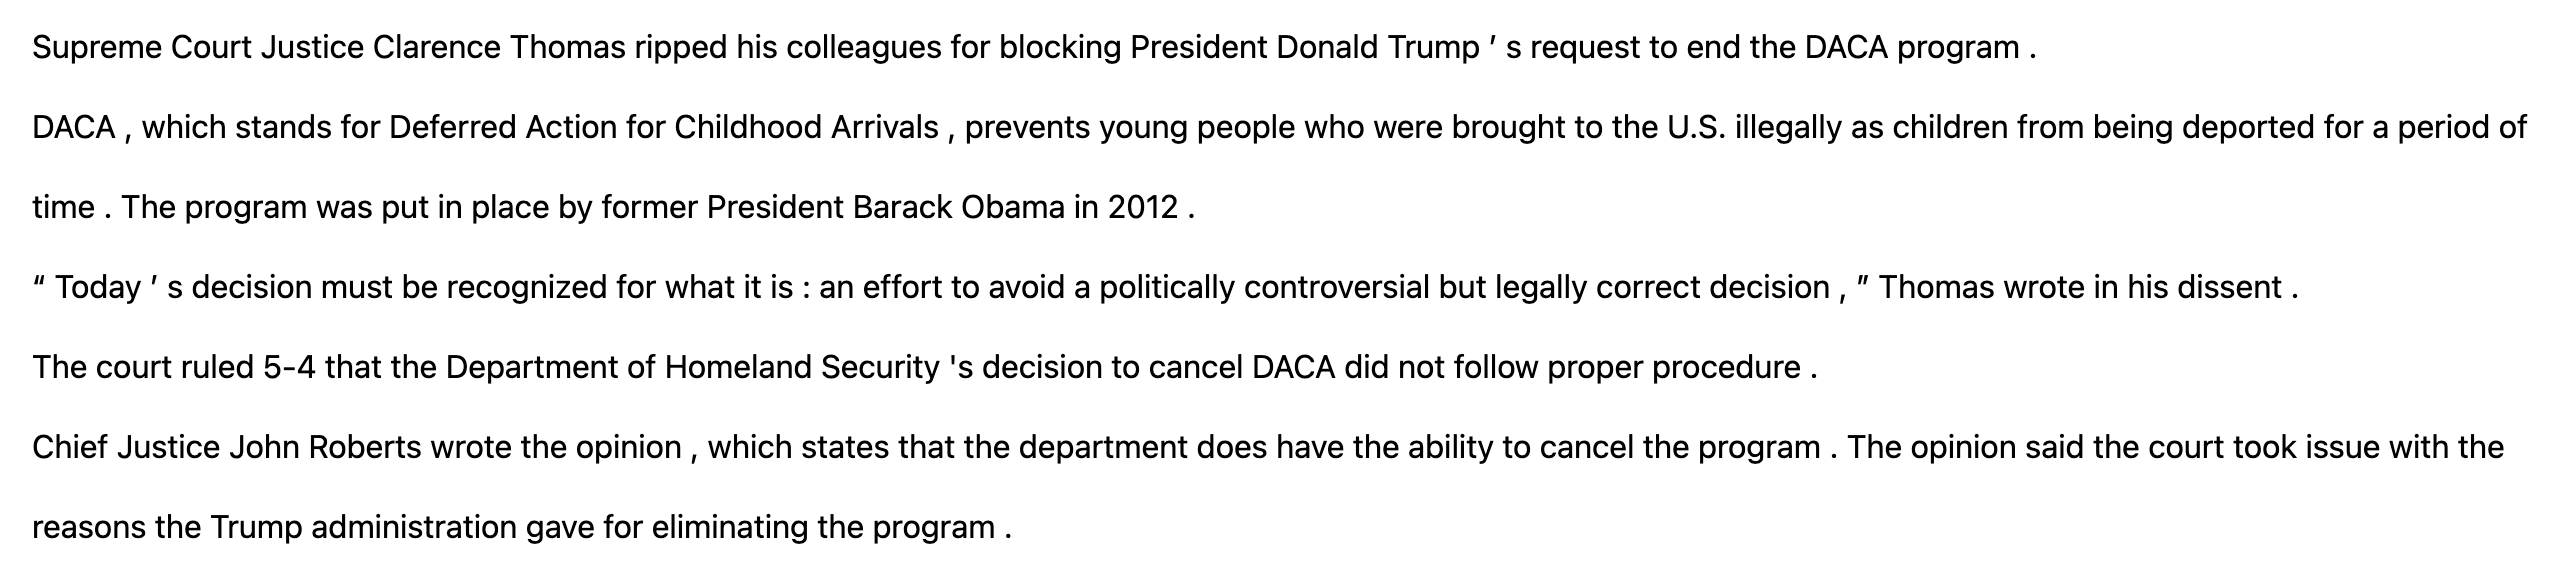
\includegraphics[width=\textwidth]{figures/article_topic_example.png}
		\caption{Text} % subcaption
	\end{subfigure}
	\vspace{1em} % here you can insert horizontal or vertical space
	\begin{subfigure}{0.3\textwidth} % width of right subfigure
		\centering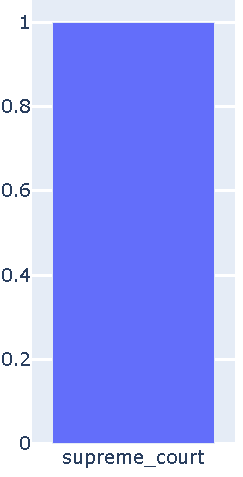
\includegraphics[width=0.5\textwidth]{figures/baly_topics.pdf}
		\caption{Native Baly topic} % subcaption
            \label{fig:topic_analysis_different_tools_baly} 
	\end{subfigure}
	\begin{subfigure}{0.3\textwidth} % width of right subfigure
		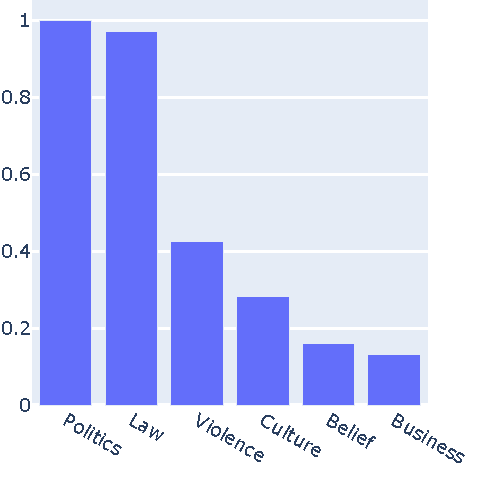
\includegraphics[width=\textwidth]{figures/coarse_topics.pdf}
		\caption{Coarse Topics} % subcaption
            \label{fig:topic_analysis_different_tools_coarse} 
	\end{subfigure}
	\begin{subfigure}{0.8\textwidth} % width of right subfigure
		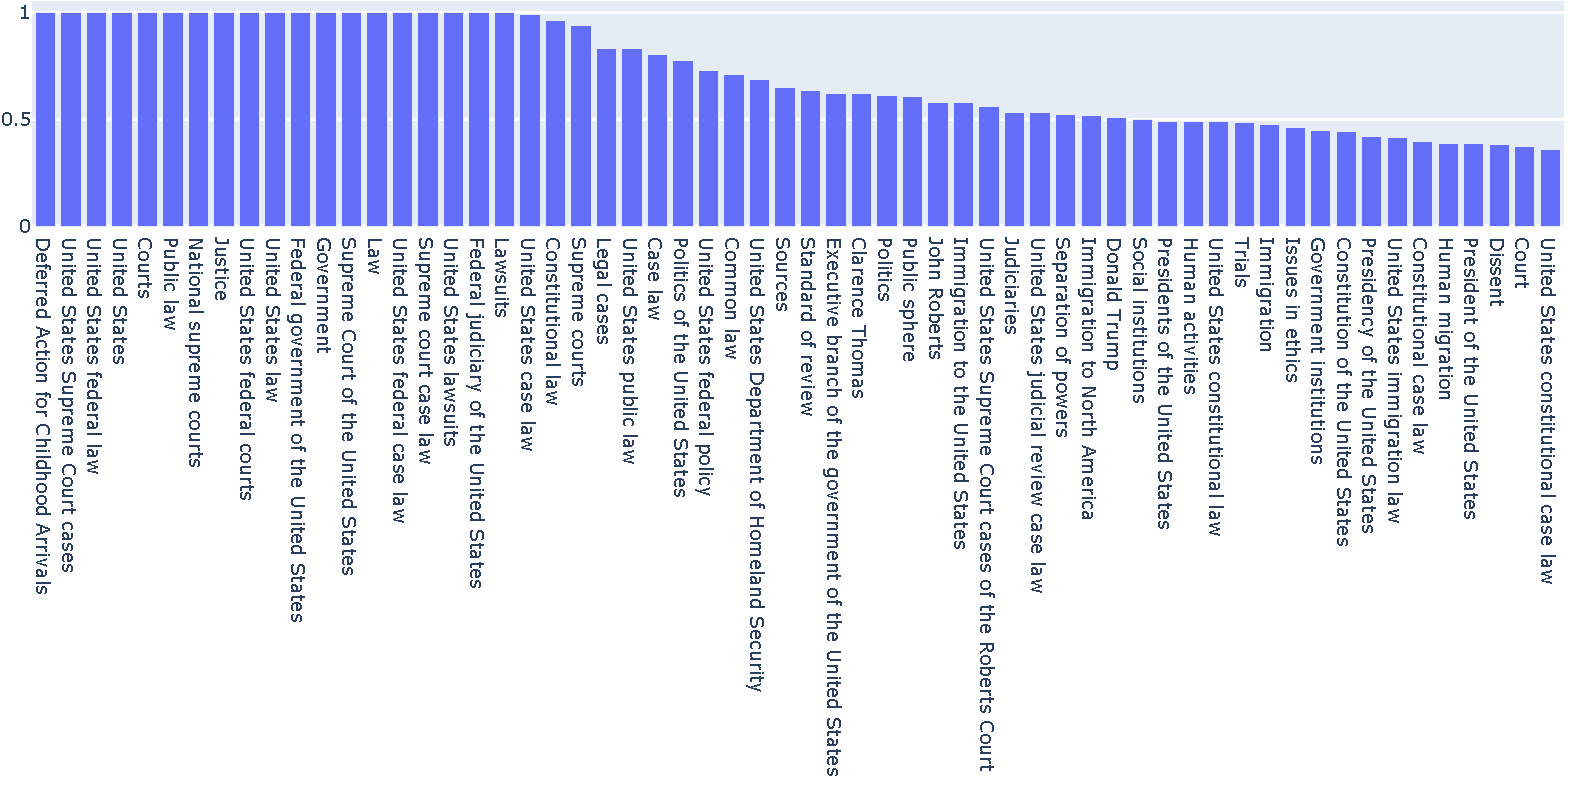
\includegraphics[width=\textwidth]{figures/finegrained_topics.pdf}
		\caption{Fine-grained topics} % subcaption
            \label{fig:topic_analysis_different_tools_fine} 
	\end{subfigure}
	\begin{subfigure}{0.8\textwidth} % width of right subfigure
		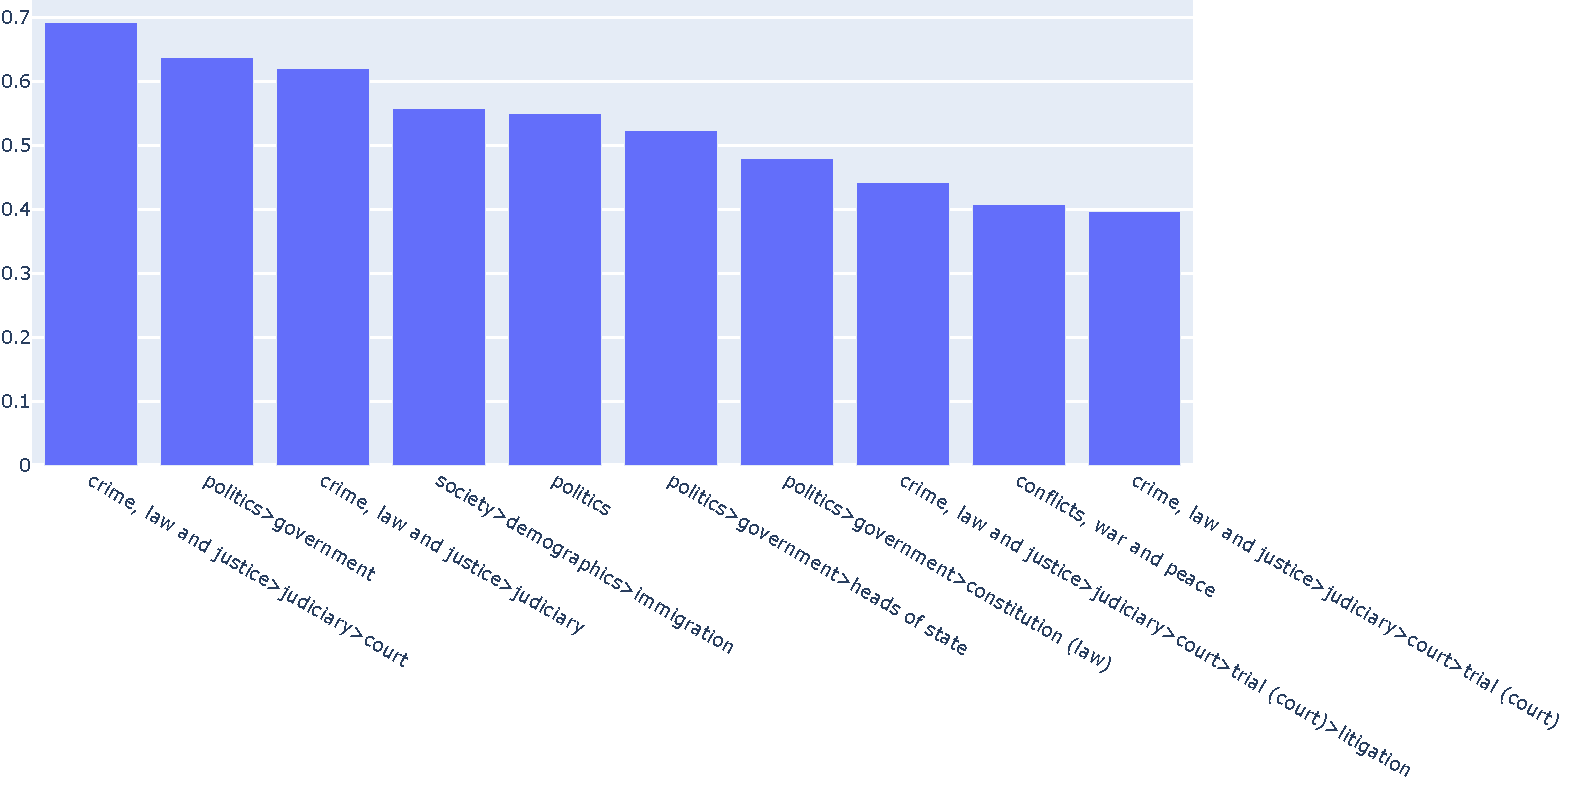
\includegraphics[width=\textwidth]{figures/mediatopics.pdf}
		\caption{Mediatopics} % subcaption
            \label{fig:topic_analysis_different_tools_mediatopics} 
	\end{subfigure}
    \caption{Different topic analysis}
    \label{fig:topic_analysis_different_tools} 
\end{figure}

Figure~\ref{fig:topic_analysis_different_tools} shows an example of these features for an article.\footnote{\url{https://www.newsmax.com/politics/clarence-thomas-daca-illegal-immigrants-dhs/2020/06/18/id/972897/}} We can see that the native topic annotations provided by the dataset have a single topic (supreme court), which is a non-standardised topic. These annotations from the dataset suffer from undefined granularity (it is not stated how coarse each topic is, there are wide topics e.g., politics, together with very narrow ones) and undefined enumeration (it is unclear the set of possible labels, topics not decided a priori).
Then we have the coarse topics, which are 6 topics that are very broad. Then the fine-grained topics, that here we only display the top 60 but there are 270 for this article. And finally the mediatopics, that are up to 10 for each article and they are part of a taxonomy and therefore we can see how specific / and what the parent topics are.

% , but in this chapter we focus on the results given by TextRazor.
% TextRazor gives topics in different ways:

In Sections~\ref{sec:topic_topic_granularities} (\ref{ssec:topic_topic_granularities_alone} and~\ref{ssec:topics_topics_leaning}) we use the selected methods to provide statistics of the \texttt{baly} dataset across topics and across leanings. In this way, we also give an insight in the methods themselves. In this way, we decide which of the methods is better for our comparative analysis.

\subsection{\statusorange Combining the analysis of dimensions}
\label{sec:topic_method_combining}
\todo{Methdology, describe better}

Having the annotations related to three different dimensions (propaganda/leaning/topic), the next step is to perform a comparative analysis bringing the dimensions together.
we compare them to understand what varies between the different topics, combining them gradually with the other two dimensions (propaganda and leaning).


% \subsection{Linking the experiments together}
% \label{sec:topic_method_linking}
% How each of the following experiments is linked together



For each of the experiments, we combine differently the annotations and analyse their relationship. For the experiments in Sections~\ref{sec:topic_topic_granularities}, \ref{sec:topic_propaganda} and \ref{sec:topic_propaganda_leaning}, we observe the differences when applying different partitioning of the dataset (based on the chosen annotations). For experiment in Section~\ref{sec:topic_classifier_propaganda}, we instead use the annotations of the topic to break down the results of the political leaning classifier of the previous chapter.

% description of each experiment
TODO: type 1 and type 2, then hierarchically all the experiments

Topic analysis at different granularities:
coarse topics, fine-grained, hierarchical. We need hierarchical topic that can go into detail because high-level topics are very broad and distributions are not very meaningful. We need to take a closer look at the details, but as well to understand where these detailed topics stand in the larger picture. (RQ1)

Topic analysis across political spectrum:
Coarse topics are very similar across political spectrum
Fine-grained topics are slightly different (quantity, terms). Which ones? They express the choice of details that we discussed in chapter 3

PROPAGANDA and Topic: only considering hierarchical topics.
Which topics contain more detected propaganda?
How detected propaganda varies across topics? 

Propaganda and Topic and Leaning:
Which topics have propaganda that differs the most across the spectrum? (Quantities of techniques/terms/) Measured with the correlation of (propaganda features) between Left and Right.
Do some of the findings clash with the “knowledge of the context”/”what should happen”? These topics may be the problem for propaganda detection
Political Leaning Classifier with Propaganda features: adding Topic
Breakdown of F1 measure across topics. Not train/test but just looking at the models trained in the previous chapter and seeing which topics were more easy/difficult to predict. We cannot train a classifier with 50/100 articles.



% \section{Topic analysis}
% \label{sec:topic_topic}

% Why: understand which practical definition of topic is better for our analysis. Granularity, type, ...

% How: First we recall the definition of topic that we gave in Chapter~\ref{sec:lit_topics} and the computational approaches that are mostly used.

% \subsection{Topic definition}
% \label{sec:topic_topic_def}

% What it is:
% - categories / groups 
% - refer to chapter 2 briefly

% How it relates to concepts described in this thesis:
% - headlines, clusters
% - topic and anti-topic layers/words: refer to Chapter~\ref{ssec:lit_layers_of_info}

% \subsection{Computational Approaches}
% \label{sec:topic_topic_computation}

% \todo{Everything here goes in chapter 2}

% Explain here different tools/methods that provide topics/entities

% We have approaches that try to determine the topics without having external knowledge, and approaches that instead an existing taxonomy/list of topics and try to map the input documents to them.

% \subsubsection{LDA topics}

% One of the most common methods to extract topics is to ``automatically detecting them" from the corpus.
% The idea is to learn from the data and by selecting a specific number of output topics, we get them.
% Problem: difficult to extract labels

% The problem of assigning labels: can we really tell what is different about the groups?
% Need to know beforehand how many topics we want in output.
% TODO

% Topic identification is a method for identifying hidden subjects in enormous amounts of text1. It can help you find common themes or keywords that represent the main ideas of a document or a collection of documents. For example, if you have a set of news articles, you can use topic identification to find out what are the most discussed topics among them.

% One of the techniques for topic identification is called Latent Dirichlet Allocation (LDA)12. It is a statistical model that assumes that each document is composed of a mixture of topics, and each topic is composed of a distribution of words. LDA can learn these topics and words from the data without any prior knowledge or labels. LDA can be implemented using Python’s Gensim package1, which provides various tools for natural language processing.

% LDA is a type of topic modeling that uses a latent Dirichlet allocation approach12. Topic modeling is a form of unsupervised learning that can be used for exploring unstructured text data by inferring the relationships that exist between the words in a set of documents23.

% LDA assumes that each document is composed of a mixture of topics, and each topic is composed of a distribution of words13. LDA can discover topics that are hidden (latent) in a set of text documents by inferring possible topics based on the words in the documents34. LDA uses a generative probabilistic model and Dirichlet distributions to achieve this4.

% Another technique for topic identification is called bag-of-words2. It is a simple way to represent text data as a collection of words and their frequencies. Bag-of-words ignores the order and structure of sentences, but it can capture some basic information about the content and vocabulary of a document. Bag-of-words can be used with simple NLP models such as TF-IDF or Naive Bayes to identify topics from texts.


% \subsubsection{Entity Annotators}
% DBPedia spotlight: entity annotation is not very good. It struggles to recognise all the entities in the articles (proof?) → DISCARDED
% BLINK (Facebook): huge (30GB models to fit on RAM), not running on my laptop. On server: no NVIDIA drivers (wants GPU) → DISCARDED
% Spacy-entity-linker https://github.com/egerber/spaCy-entity-linker/ . Not very widely used. → DISCARDED

% Then from entities, need ways to derive the topics by navigating knowledge bases (wikidata in most cases)

% \subsubsection{TextRazor}
% TextRazor: seems more accurate, industrial, FreeBase taxonomy. Each entity is annotated with wikidata id and a list of FreeBase types. Also provides topics and fine-grained topics

% benchmarks? check that it is better than other tools
% % Regarding the validation of TextRazor, I am not aware of a benchmark done to check if it is better than other tools. It was suggested by Harith to use it, and I find that the data it provides is generally quite good (for topics and entities). But this is qualitative, I didn’t do a benchmark or looked up for benchmarks. The assumption was that it’s a commercial product and it should be good.
% some papers that claim to do benchmarks:
% http://giusepperizzo.github.io/publications/Rizzo\_Erp-LREC2014.pdf for the entities
% https://www.linkedin.com/pulse/google-nli-kill-market-linguistic-apis-review-yuri-kitin/ mentioning that TextRazor is useful because it links to Wikipedia/DBPedia

% TextRazor is the only one that provides already hierarchical topics, the other ones always give topics that are not hierarchical or can be made hierarchical with external knowledge (e.g. using DBPedia to navigate broader topics).

% What it provides



\section{\statusorange Topics for Comparative Analysis}
\label{sec:topic_topic_granularities}

In this section, we use the different topic methodologies listed above, applying them to the \texttt{baly} dataset.

Our goals are many:

\begin{itemize}
    \item analyse the dataset to understand the topic it contains, using different methodologies;
    \item compare the information provided by each methodology and understand what are the advantages of using one or the other;
    \item see which methodologies are able to find differences between Left and Right. The dataset itself is made of triples of articles, so we expect that the high-level topics will be very similar, and instead, we expect some fine-grained differences.
\end{itemize}

Therefore, we divide this section in two main parts: the first one, Subsection~\ref{ssec:topic_topic_granularities_alone}, contains the analysis of the topics of the dataset, with the different methodologies. The second part, Subsection~\ref{ssec:topics_topics_leaning}, contains a comparative analysis of the topics with respect to political leaning.

We end this section with~\ref{ssec:topic_topic_choice} which recaps and motivates our choice of hierarchical topic methodology for the next sections.

% This contains 3.1 (topic alone) and 3.2 (topic + leaning).
% This section has to support the need for hierarchical topics.
% We want to analyse differences across topics and granularity is required to be able to inspect at different levels.
% Only top-level topics are not good because they don't show good differences.

% Here we take different topic definitions and we try them to show that we need granularity.

\subsection{\statusgreen Detected Topics in the Dataset}
% \subsection{Detected Topics at different granularities}
\label{ssec:topic_topic_granularities_alone}
% ONLY TOPIC
% Why: understand which practical definition of topic is better for our analysis. Granularity, type, ...

% How: First we recall the definition of topic that we gave in Chapter~\ref{sec:lit_topics} and the computational approaches that are mostly used.

% analysis of baly dataset at different granularities

% RQ1 (NO): How can we optimise the definition of the topic in order to have enough details? 


% GOAL
Given our goals 1 and 2, we want to compare the information that different methodologies can provide about a selected dataset. Some techniques may be better to provide general information while others may provide very fine-grained topics.

% what
As described in the Methodology section (Section~\ref{sec:topic_method}, we consider the \texttt{baly} dataset and we apply different topic labels.

In the following paragraphs we consider:

\begin{enumerate}
    \item AllSides native topics
    \item Coarse Topics (TextRazor)
    \item Fine-Grained Topics (TextRazor)
    \item Hierarchical Mediatopics (TextRazor)
\end{enumerate}

% We start with the definition of topics that is contained in the Baly dataset, and then we use the different topic types that we get from TextRazor, starting with simple ones to get to the more complex.

\subsubsection{\statusgreen Custom topics (AllSides)}

The first topic definition that we apply is the ones that comes directly from the \texttt{baly} dataset. Toghether with the triples of articles, available from their website, the AllSides headlines have a manual annotation of the topic, which is given by the editors. In this way, the users can filter by topic and find related information.
Besides being useful for navigating the website, this is a useful label because it is given directly by the resource creators and not assigned externally.
This attribute is then collected in the \texttt{baly} dataset and we have it available.

A complete list of the topics can be found on the AllSides website.\footnote{\url{https://www.allsides.com/topics-issues}}

\begin{figure}[!htbp]
    \centering
    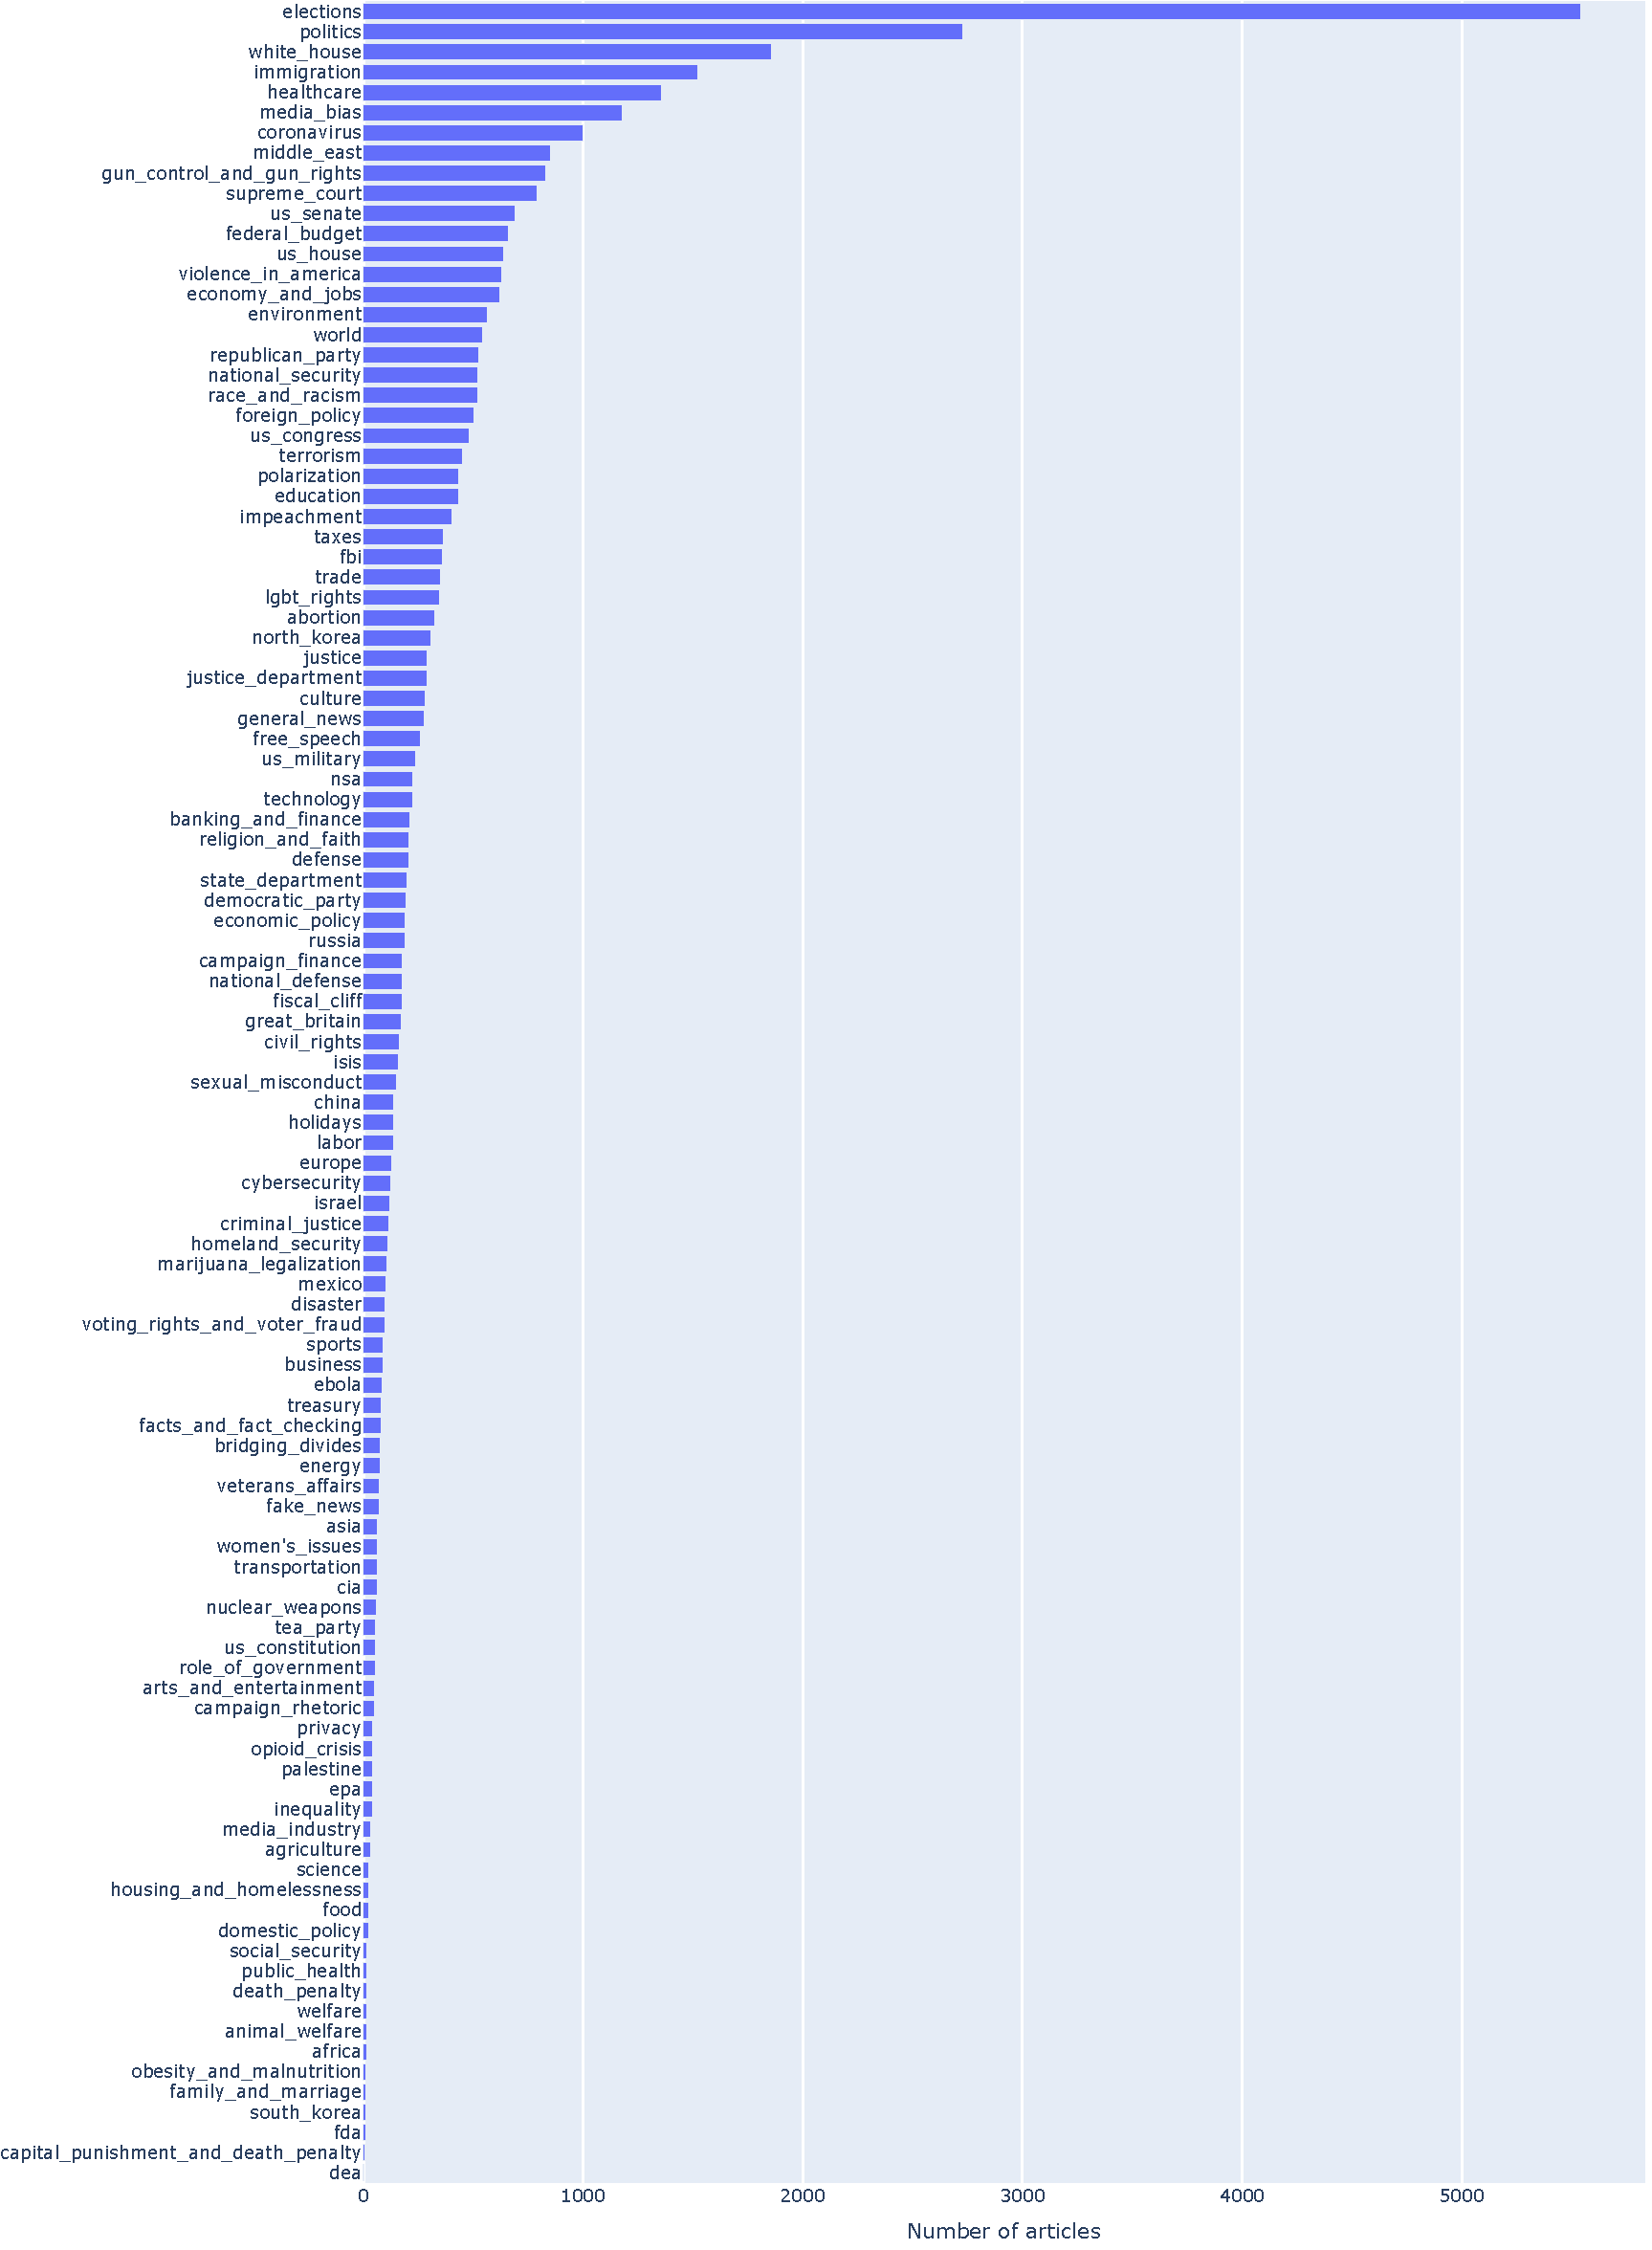
\includegraphics[width=\linewidth]{figures/baly_original_topics.pdf}
    \caption{Original topics of \texttt{Baly} dataset}
    \label{fig:baly_original_topics}
\end{figure}

In Figure~\ref{fig:baly_original_topics} we can see a histogram of the topics. We can make several observations:

\begin{itemize}
    \item the labels of the topics are not uniform in terms of granularity: there are some very wide topics (e.g., politics) and some very narrow ones (e.g., DEA);
    \item the labels are annotating several aspects and having only one label per article this means that some articles are annotated for the location mentioned (e.g., world, Africa, Russia, Asia, South Corea) while others for more ubiquitous topics (e.g., immigration, healthcare, environment, economic policy, civil rights); % traversal (food, privacy, healthcare, …)
    \item the distribution are very unbalanced across topics: election has more than 5k articles, while DEA has only a few;
    \item some topics are subtopics of other ones (e.g. electionss is a subtopic of politics) but no information about the relationships is provided;
    \item with 108 flat topic it becomes difficult to compare and organise the topics.
\end{itemize}

An improvement could be done by analysing these labels and manually establishing the relationships, to organise hierarchically the topics.

% Pro: defined by the authors, by hand
% Cons: hierarchically disomogeneous, highly imbalanced

% Original topics
% The dataset is provided together with topic labels but they have a big problem: they are annotated with labels that have very different granularities.
% 108 topic labels
% Most frequent topics: elections, politics (very general), white house, immigration, healthcare
% Least frequent topics: dea, capital punishment and death penalty, fda, south corea
% Labels are not uniform:
% In granularity: e.g., elections vs politics, one is a subtopic of the other
% In aspect: e.g. geography (south corea, africa, china, russia) vs more generic and traversal (food, privacy, healthcare, …)


These topic labels are given by the AllSides team with an unknown criteria, and the above shows how diverse and not-uniformed they are.

For this reason, the next paragraphs consider standardised topics instead of ad-hoc topics.


\subsubsection{\statusgreen Coarse Topics}

In this section we take into consideration the TextRazor coarseTopics annotations. TextRazor is a commercial API that allows to analyse topics, entities and to perform other NLP-related tasks (e.g. classify documents, …).
Regarding the topics, it provides the Coarse Topics, which are 16 very high-level topics (Belief, Business, Culture, Education, Health, Language, Law, Leisure, Mathematics, Nature, Politics, Science, Sports, Technology, Violence, Weather).
Each document is assigned with the top 5/6 matching Coarse Topics, each one with a relevance score which ranges in $[0,1]$. Those scores don’t sum to 1. Each document is assigned to multiple topic, not a single one (multiclass).

For this reason, we explore the topics in two different ways:

\begin{enumerate}
    \item considering the most important topic for each article: this is simpler, each article corresponds to a single topic.
    \item considering the topic weights: each topic corresponds to multiple topics with a specific weight.
\end{enumerate}

\paragraph{Most relevant topic Only}

For this first simplification, each article is associated to its most representative topic. This means that if an article is annotated with a score of $1.0$ to Politics and with $0.9$ to Culture, it will only count for Politics because all the topics from second position onwards are discarded.


\begin{figure}[!htbp]
    \centering
    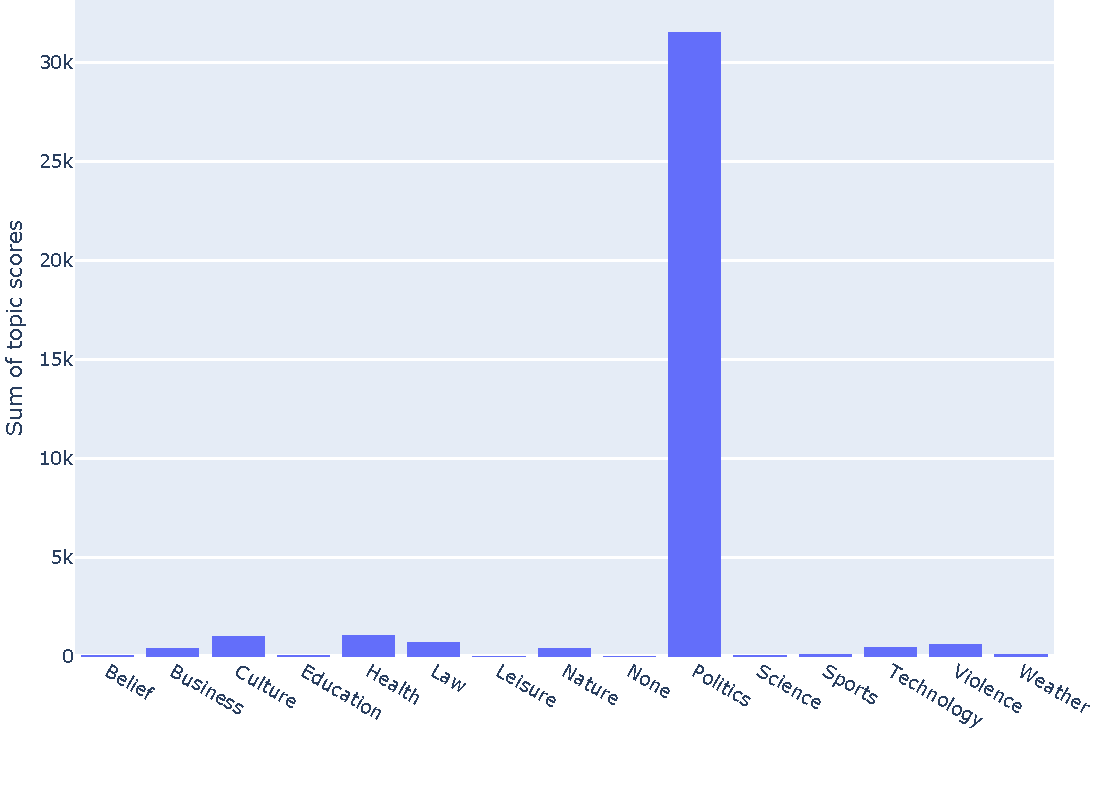
\includegraphics[width=\linewidth]{figures/baly_coarse_first.pdf}
    \caption{Coarse Topics most relevant of \texttt{Baly} dataset}
    \label{fig:baly_coarse_first}
\end{figure}

In Figure~\ref{fig:baly_coarse_first} we can see how the articles distribute across topics when only considering the most important one.

This shows that the dataset is highly unbalanced on Politics. This makes this specific usage of the topic annotations highly unusable.

The main problem is that we can only see that the dataset is centred about politics, but all the secondary topics are suppressed.
This plot does not give further insights.
Also, we can see that two of the high-level topics do not even exist for a single article (Language and Mathematics).

This analysis is the result of an oversimplification.

\paragraph{Weighted (multi-topic)}

For this reason, we decide to use all the topics for an article and not only the most important one.
If we consider each of the 5/6 topic for each article, we can also see topics which are still very important and may have been discarded only because politics was slightly higher.

\begin{figure}[!htbp]
    \centering
    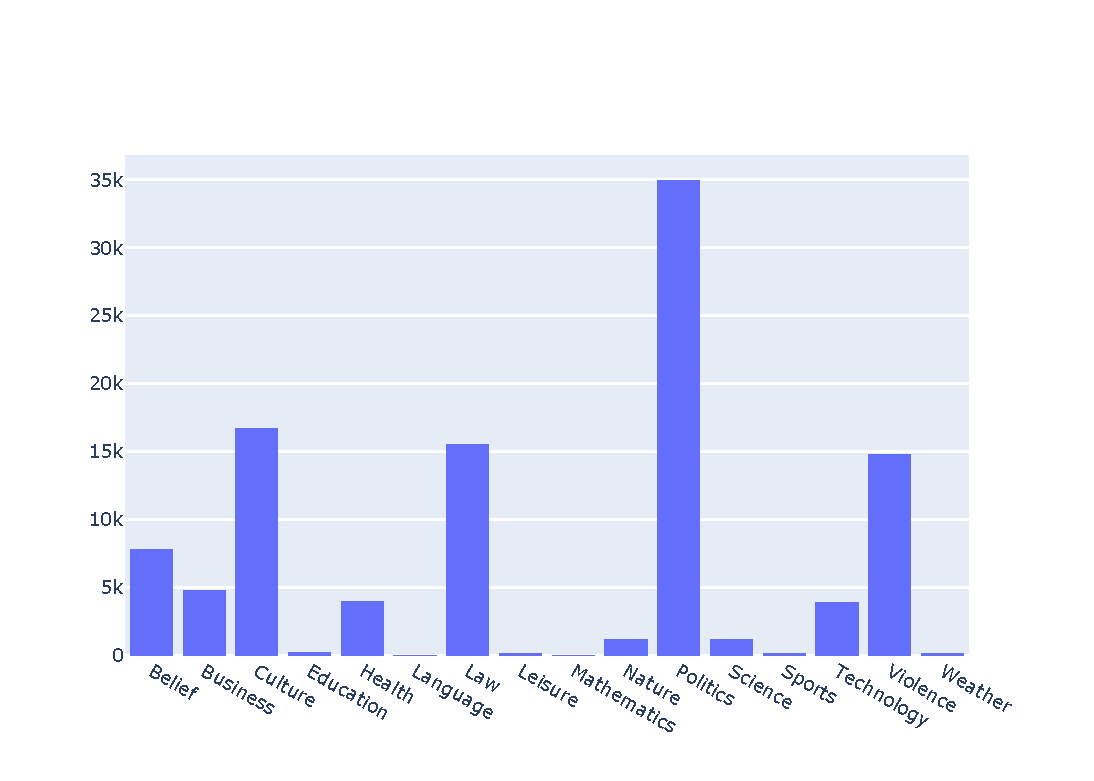
\includegraphics[width=\linewidth]{figures/baly_coarse_weighted.pdf}
    \caption{Coarse Topics weighted of \texttt{Baly} dataset}
    \label{fig:baly_coarse_weighted}
\end{figure}

Figure~\ref{fig:baly_coarse_weighted} shows that the distribution over topics contains more topics other than Politics.
Still, Politics is the most relevant, but we have as well Culture, Law and Violence that appear in a significant number of articles.

To produce the values displayed in Figure~\ref{fig:baly_coarse_weighted}, we sum the individual scores given to each article and topic. The scores being a value in the $[0,1]$ range, the vertical axis does not represent the number of articles that have a specific topic, but instead represents the sum of the scores. The total number of articles is $37,554$.
%For example, considering that the total number of articles in the dataset is 37,554, we can see that around 35k 

% We can see that the distribution is slightly unbalanced towards politics, then culture, law and violence. This looks like the topics are not too unbalanced, but we have to remember that we would like to have a single document to be categorised only with one topic, and this is not the case.

With respect with the previous Figure~\ref{fig:baly_coarse_first}, we can understand better the topics that the dataset contains.
Still, the topics are very high-level and we do not have insights about which political issues are discussed, or which law subtopics are contained.



\subsubsection{\statusorange Fine-Grained Topics}

Moving to the next topic feature, we analyse the annotation that TextRazor provides for Fine-Grained Topics.

As we saw in subfigure~\ref{fig:topic_analysis_different_tools_fine}, the fine-grained topics are very specific and for each input article, the annotations provide a variable number of them, also some hundreds.
Fine-grained topics are somewhat similar to mentioned entities, given the high number of matches for each of the articles. Differently from entities, they are not bounded to a specific occurrence in the text (for entities we are able to get the character offsets of the article, to know which words evoke the entities) and an article may contain a fine-grained topic even if the topic name is not  mentioned in the article.

Across the whole \texttt{baly} dataset, we have $98,504$ distinct fine-grained topics, and it becomes very difficult to present some statistics or graphical representations given this huge number.

It is good to have fine-grained information that is very specific, but at the same time it is unclear how to link the fine-grained information to the high level topic. What we are missing is some relationship between the two levels, that may possibly be hierarchical with multiple levels.
With a hierarchy, we can adaptively decide the level of detail and find the optimal one between topics that are too broad (coarse topics for example) and too narrow (fine-grained topics).

% Baly dataset: 99941 fine-grained topics overall
% Example:
% TODO FIGURE MONGO TOPICS

% annotated only at the article level (not possible to align with propaganda techniques)
% Many distinct: 98.504
% At this point maybe we could directly use the entities which have a word-level annotation 


% find some of them that are specific of a political leaning? 

\paragraph{\statusred Potential ways to aggregate and find middle-level topics}
\todo{improve this paragraph}

To potentially aggregate the topics and find a slightly higher level of hierarchy, there are different solutions.

The topics have in their attributes the \texttt{wikidata\_id} that is useful to link to Wikidata. Wikidata is useful to see the types of the entity and other relationship types.

For example, the relationships \texttt{instance\_of} and \texttt{subclass\_of} provide links to wider topics. In theory, every type of relationship is important: e.g. ``Trump Wall" Q61989464 is \texttt{named\_after} Donald Trump.

Or by using the \texttt{WikiLink}, it is also possible similarly to use the categories tree (in reality it’s a Graph) of Wikipedia.\footnote{ \href{https://en.wikipedia.org/wiki/Special:CategoryTree?target=Category\%3APolitics&mode=all&namespaces=&title=Special\%3ACategoryTree}{https://en.wikipedia.org/wiki/Special:CategoryTree}}

In both ways, the upper categories are many for each node, and it’s quite difficult to get a clean taxonomy.

There exist some previous works that addressed this problem.
cleaning up relationships to extract pages+categories taxonomy.

WiBi taxonomy → http://wibitaxonomy.org/ dead Wikipedia Bitaxonomy Explorer
\cite{flati2014wikipedia,flati2014two,ponzetto2009large}

\cite{chu2019tifi} for fictional domain, cleaning up category graph for fictional domains

% Backlinks? What are they?

% Wikipedia categories github experiment? https://github.com/wasiahmad/mining\_wikipedia/tree/master/WikiNomy 



% Reduction to different granularities of topics:
% Wikidata IDs → wikidata embeddings? (too difficult, also to explain the features and analysis / explanation)
% Wikidata ← → link to IPTC topics (offered by IPTC, handmade by them)
% For each entity, navigate its triples to find IPTC topics. Relationships of type:
% Instance\_of
% Subclass\_of
% ???
% In theory, every type of relationship is important: e.g. “Trump Wall” Q61989464 is “named after” Donald Trump 


% Trying to find topics that are not so tight
% https://en.wikipedia.org/wiki/Wikipedia:Contents/Categories 
% This number of topics is too high. How to climb a bit up the topic tree in Wikidata?
% wikidataId → entity. From the entity navigate the relationships instance\_of and subclass\_of. But also other relationships could be useful?
% From WikiLink → wikipedia page. From the page navigate the categories (recursively) to climb up the categories tree (in reality it’s a Graph) of wikipedia \url{https://en.wikipedia.org/wiki/Special:CategoryTree?target=Category\%3APolitics&mode=all&namespaces=&title=Special%3ACategoryTree}
% In both ways, the upper categories are many for each node, and it’s quite difficult to get a clean taxonomy.
% Previous works:
% https://www.academia.edu/download/30772075/ponzetto\_slides.pdf cleaning up relationships to extract pages+categories taxonomy.
% https://aclanthology.org/P14-1089.pdf WiBi taxonomy → http://wibitaxonomy.org/ dead http://ceur-ws.org/Vol-1272/paper\_81.pdf https://aclanthology.org/P14-1089.pdf https://www.diag.uniroma1.it/navigli/pubs/IJCAI\_2009\_Ponzetto\_Navigli.pdf 
% https://dl-acm-org.libezproxy.open.ac.uk/doi/abs/10.1145/3308558.3313519 for fictional domain, cleaning up category graph for fictional domains

% Backlinks? What are they?

% Wikipedia categories github experiment? https://github.com/wasiahmad/mining\_wikipedia/tree/master/WikiNomy 
\paragraph{\statusred A badly structured problem}
\todo{improve this paragraph}

Some sentences here, to say that topic taxonomies already exist, and it is better to directly recognise topics using the taxonomies.


% \paragraph{With IPTC}
% So let’s take all the relationships and navigate some hops until an IPTC topic comes up (termination).
% Feature building: decay with the number of hops the weight (exponentially? 1, 0.5, 0.25, …) of each entity.
% Table of entities (quite many distinct), with filter on number of appearances

% \paragraph{Without IPTC}

% We can just take a look at the fine-grained topics:
% Minimum support filter (to reduce features) or select top-k topics

% Option with linked entities:
% Don’t lose a lot of fine-grained topics/entities which don’t have enough support
% Consider them with the related entities in KB
% How to do this: 
% Navigate hops from each entity (decay weight)





% \subsubsection{Derived from Entity types}
% \todo{remove this?}

% Freebase Taxonomy revised by TextRazor

% entity propaganda feature computation
% For each entity, compute the total/average propaganda techniques that co-occur in the same sentence %by each political leaning.
% E.g.: “Donald Trump” used a lot of times with “Doubt” % from the Left leaning.

% Interesting direction:
% With Entity linking (provided by TextRazor) it is possible to find common attributes of the entities that make them targets of %Left/Right 
% propaganda. E.g., a category of people as repeated target of Propaganda

% \paragraph{filter the entities types}

% Using all the entities is too much.

% Option 1: choose the types that will be mostly framed differently by Left/Center/Right (related to politics and sensitive topics e.g. Wikipedia list/ Allsides List
% Option 2: automatically discover the types that are featured more differently from L/C/R in the training dataset

% \paragraph{FreeBase Taxonomy and TextRazor}

% FreeBase vs TextRazor

% Analysis of the types listed in FreeBase
% TextRazor: https://www.textrazor.com/blog/2015/10/freebase-type-deduction-with-data.html they took freebase and are continuing to update it.
% FreeBase build taxonomy: path-like. Let’s build the tree from the path pieces (e.g. /Location/Country is a child of /Location)
% Interesting types: religion, military, law, business, organisation, government, location/country, people (how to justify?)

% Freebase Taxonomy (revised by TextRazor): https://drive.google.com/file/d/145CpFSFA0\_kuzvNt4z\_H1F2nKi-9-YyF/view?usp=sharing 
% Entities types appearing on the headlines dataset: https://drive.google.com/file/d/166fz78O\_xKesnCQ\_hDGiLSH5jk8WdV86/view?usp=sharing 




\subsubsection{\statusgreen IPTC Media Topics}

To solve the problems identified (the topics are either too coarse-grained or too fine-grained, without link between them), we decide to analyse the dataset with a topic taxonomy.

Between the many taxonomies for topics (e.g., scientific publications, ...TODO), we focus on the news domain and therefore the most important and used taxonomy is IPTC NewsCodes Media Topics.
This is a taxonomy especially created to describe the topics of news articles. It is made of 17 top-level terms, that can be expanded up to 5 levels of subcategories.
The full taxonomy can be seen at \url{https://cv.iptc.org/newscodes/mediatopic} and an interactive display at \url{https://show.newscodes.org/index.html?newscodes=medtop&lang=en-GB&startTo=Show}.

% Problem: very difficult to group fine-grained topics into more wide ones
% Solution: IPTC NewsCodes Media Topics schema https://cv.iptc.org/newscodes/mediatopic/
% It’s a taxonomy (5-levels categories)
% TextRazor also provides mediatopic if request is performed with appropriate parameters.

% https://iptc.org/news/wikidata/ 
% TreeView: \url{https://show.newscodes.org/index.html?newscodes=medtop&lang=en-GB&startTo=Show}

% https://cv.iptc.org/newscodes/mediatopic/
% 17 top-level terms
% 5-level taxonomy

TextRazor provides the IPTC Media Topics annotations for submitted texts, if requested with proper parameters.
As we saw in Subfigure~\ref{fig:topic_analysis_different_tools_mediatopics}, each input text is annotated with up to 10 Media Topics (with a weight from 0.0 to 1.0). For each of the Media Topics, it is possible to see the current node and the parent topics up to the top-level topics.
Therefore, it is possible to understand the relationship between the topics and get detailed information but still with the context of which more large topics this belongs to.


% Expecially developed for news
% Hierarchical


% Problem: topic is very unbalanced on this dataset (everything about “politics”)




% IPTC mediatopics
% TextRazor gives in response 10 mediatopics for each article, each one with a score

As in the previous Subsection with Coarse Topics, we consider first a simplified version where only the most relevant MediaTopic is taken, and a second version where each article is considered part of several MediaTopics.


\paragraph{Most relevant IPTC mediatopic}

For this first simplified version, each news article in the \texttt{baly} dataset corresponds to a single MediaTopic.

\begin{figure}[!htbp]
    \centering
    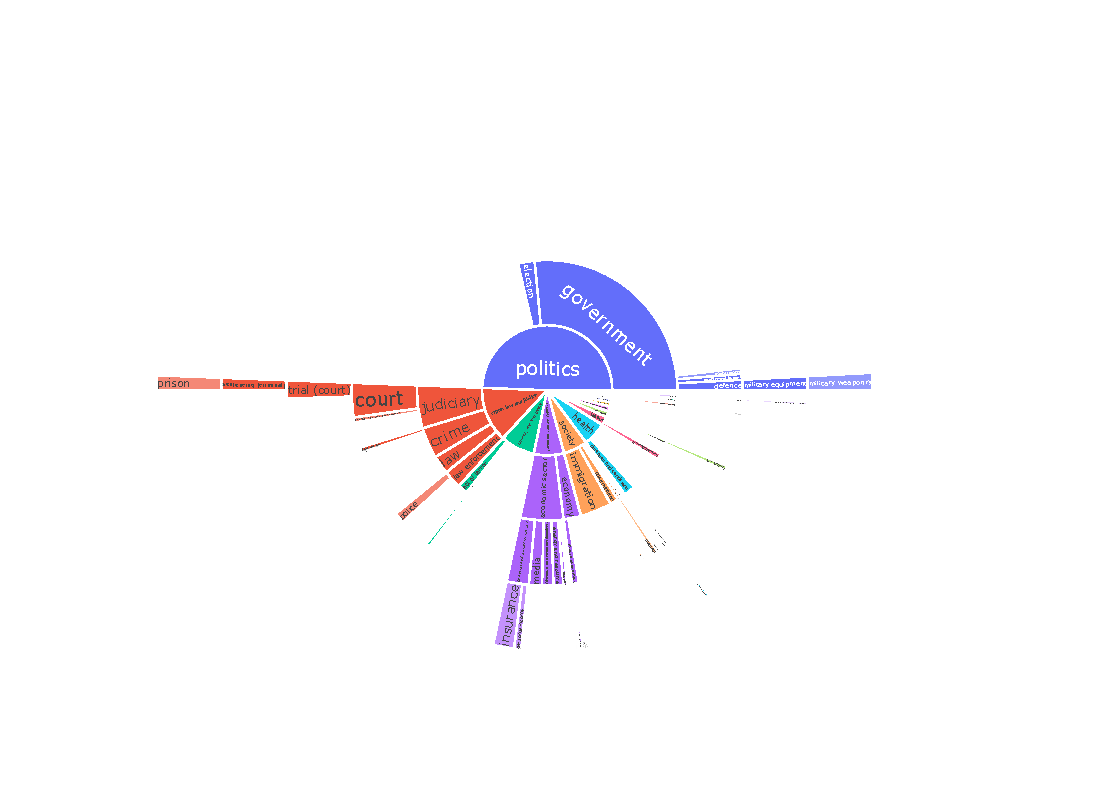
\includegraphics[trim={2.2cm 2cm 2.2cm 2cm},clip,width=\linewidth]{figures/baly_iptc_only_first.pdf}
    \caption{IPTC Media Topics of \texttt{Baly} considering only the most important MediaTopic for each article}
    \label{fig:baly_iptc_only_first}
\end{figure}

Figure~\ref{fig:baly_iptc_only_first} shows a Sunburst diagram\footnote{Interactive chart: \url{https://martinomensio.github.io/phd-project/figures/baly_iptc_only_first.html}} that represents how the most relevant topic of the articles is spread across the IPTC MediaTopic hierarchy.
In the inner circle, the top-level topic are represented (sorted by size: politics, crime-law-and-justice, conflict-war-and-peace, economy-business-and-finance) and the outer circles represent subcategories (e.g., government is a subcategory of politics, or immigration is a subcategory off society).
To build this plot, we take the most relevant mediatopic (higher score) and we add its score too the specific node in the tree. Parent nodes also receive the score, since an article that belongs to a certain subtopic, also belongs to the corresponding parent topics (up until the top level topics). The opposite is not true, and this is why summing the size of the subtopics (e.g. government + election + government policy) the total value is still less than the value for the parent topic (in our case, politics).

With respect to the previous figures of this section, we can see not only that politics is the major topic, but we can also get an idea of its main subtopics, as well as very detailed subtopics (5 levels).

However, remembering the difference between Figure~\ref{fig:baly_coarse_first} and \ref{fig:baly_coarse_weighted}, we know that this current plot is a simplification and we need to consider all the MediaTopics of each article.
We provided it because it is simpler to explain how the values for the Sunburst plot are assigned.

% Problem: only politics and government.
% How to solve: when multiple labels are given, avoid the most broad/common ones. E.g.: politics:1.0, politics>elections: 0.85 → choose elections

% What if, instead of trying dirty ways to select only one topic for each article, we keep the multi-topic annotations?
% - Each article instead of having only one topic, is a distribution over a set of topics
% - In the downstream tasks we can use this distribution as the topic description (why should it be only one topic?)
% - If we proceed in this way, we should also do the same analysis with the standard topic distribution (not mediatopics)


\paragraph{Weighted IPTC mediatopic}

By considering all the MediaTopics of each article, we have the complete picture of topics of the dataset. 

\begin{figure}[!htbp]
    \centering
    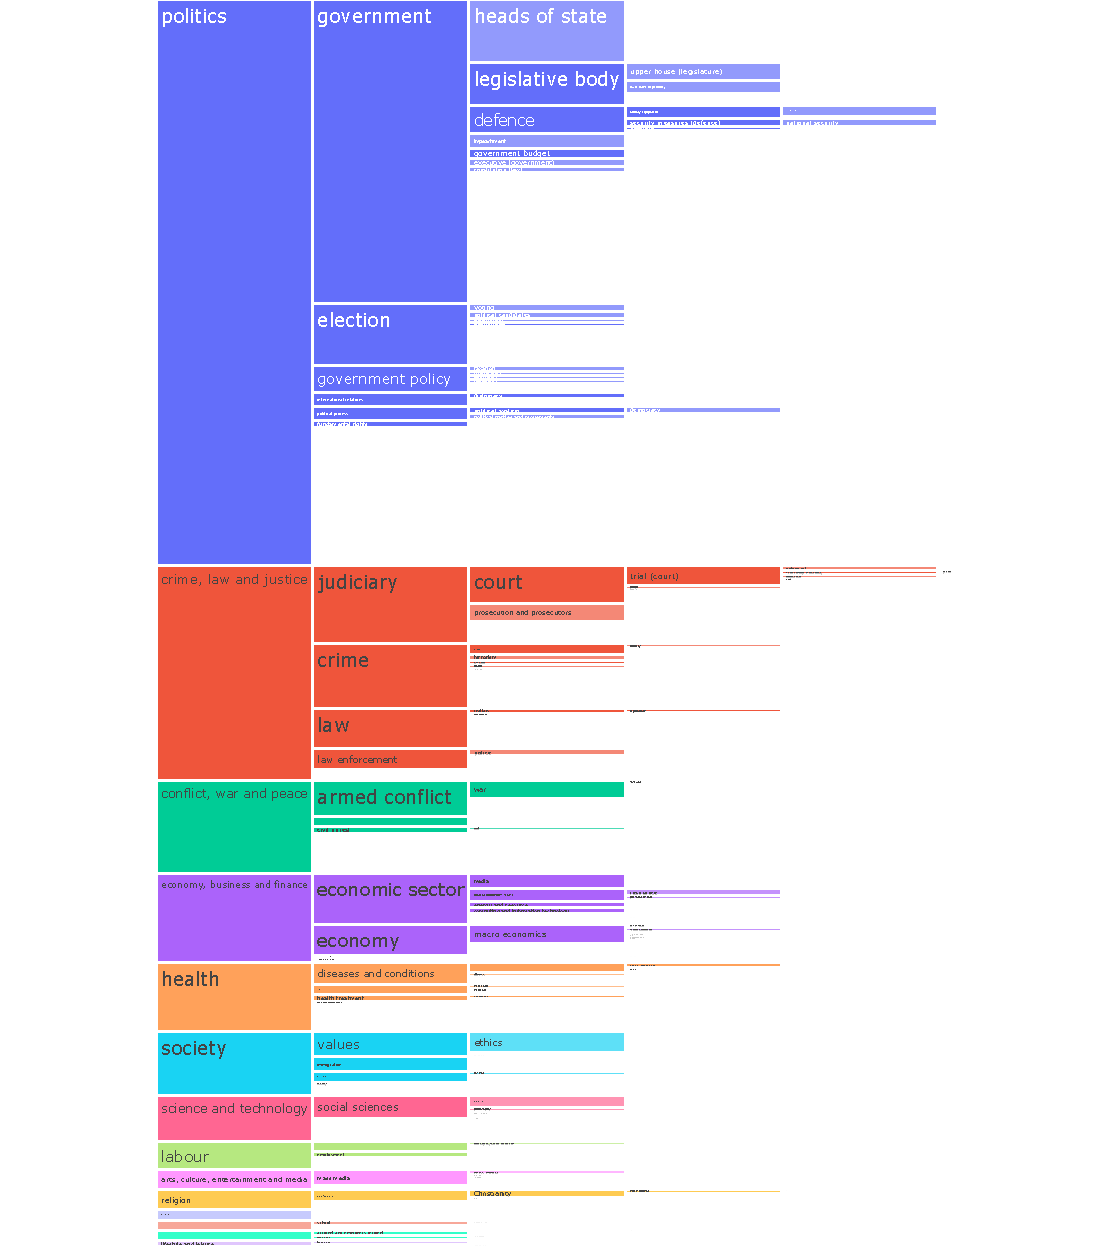
\includegraphics[trim={2.2cm 2cm 2.2cm 2cm},clip,width=\linewidth]{figures/baly_iptc_weighted.pdf}
    \caption{IPTC topics weighted of \texttt{Baly} dataset}
    \label{fig:baly_iptc_weighted}
\end{figure}

Figure~\ref{fig:baly_iptc_weighted} shows the Sunburst diagram\footnote{Interactive chart: \url{https://martinomensio.github.io/phd-project/figures/baly_iptc_weighted.html}} that is built similarly to the previous case. This time, being each article linked to multiple mediatopics, more subtopics are shown in the figure, that were suppressed by the major topic in the previous case (analogously to Fig~\ref{fig:baly_coarse_first} vs Fig~\ref{fig:baly_coarse_weighted}).

For example, under Government we see legislative-body and heads-of-state that did not appear before. Or science-and-technology and economics that were not visible before.


% Options:
% Multi-topic weighted complex solution
% Only see what happens in specific topic with the classifier
% Input topics as features and see classifier what produces:
% Need to encode the topics hierarchically
% Need model (neural network) on top that can combine the features. Single-layer neural network cannot, need 2 layers at least

% \subsection{Results}

\subsubsection{\statusgreen Comparison}

We have seen in the previous paragraphs several methods and definitions of the topic.

Simple high-level topics, show that the majority of articles are about politics. They are able to tell which topics exist, but the labels are very wide and do not provide enough detail.
On the other hand, fine-grained details can be very specific, but it is very difficult to understand how they relate with wider topics.

We analysed two different ways of using multi-class weighted labels. If we consider only the most important topic for each article, we lose a lot of information. Instead, by using all the topics, we are able to see more topics that would be hidden otherwise.

Overall, the method that gives more details and provides a context around the topic (parent topics) is the hierarchical IPTC MediaTopics considering all the topics.

We will see in the next subsection how the methods are able to provide a comparative analysis over political leaning.



\subsection{\statusgreen Topic analysis across political spectrum}
\label{ssec:topics_topics_leaning}

Having seen in the previous subsection which level of detail the different topic methodologies are able to provide, we want in this subsection to perform a comparative analysis.
We want to observe which topic differences exist across political leaning, using a dataset that is made of triples of articles.
Being groups of three articles that describe the same event, we expect that the high-level topics will be quite similar considering an article from the Left compared with an article from the Right coming from the same triple.
Therefore, also at the dataset level, the statistics at the high-level topics should be quite similar across political leaning.

What we would like to see, is some differences when we consider more narrow topics. This would link with our discussion done in Chapter~\ref{chap:common_ground_search} about the choice of details that individual news sources make, covering different subtopics to support their point of view.
Together with the leaning labels (taken from Chapter~\ref{chap:political_sides}) we want to analyse the link between the choice of subtopics and the political orientation of the news sources.

% TOPIC+LEANING: still to support that we need granularity hierarchical topics, other topics are not enough. This time taking the leaning comparison as a first use case and showing evidence that other topics are not useful to do a comparative analysis.

% Coarse topics are very similar across political spectrum
% Fine-grained topics are slightly different (quantity, terms). Which ones? They express the choice of details that we discussed in chapter 3

% RQ2: How does the topic (at different granularities) change across political leaning on a parallel news corpus?

We proceed in this subsection by considering the same methodologies for topic labelling as in the previous subsection.

\subsubsection{\statusgreen AllSides topics}

First we use the native topics included in the dataset. We simply count the number of articles for each leaning and topic. Our goal is to see how balanced they are across leaning, and if there are some topics which have more articles on a specific leaninig.

\begin{figure}[!htbp]
    \centering
    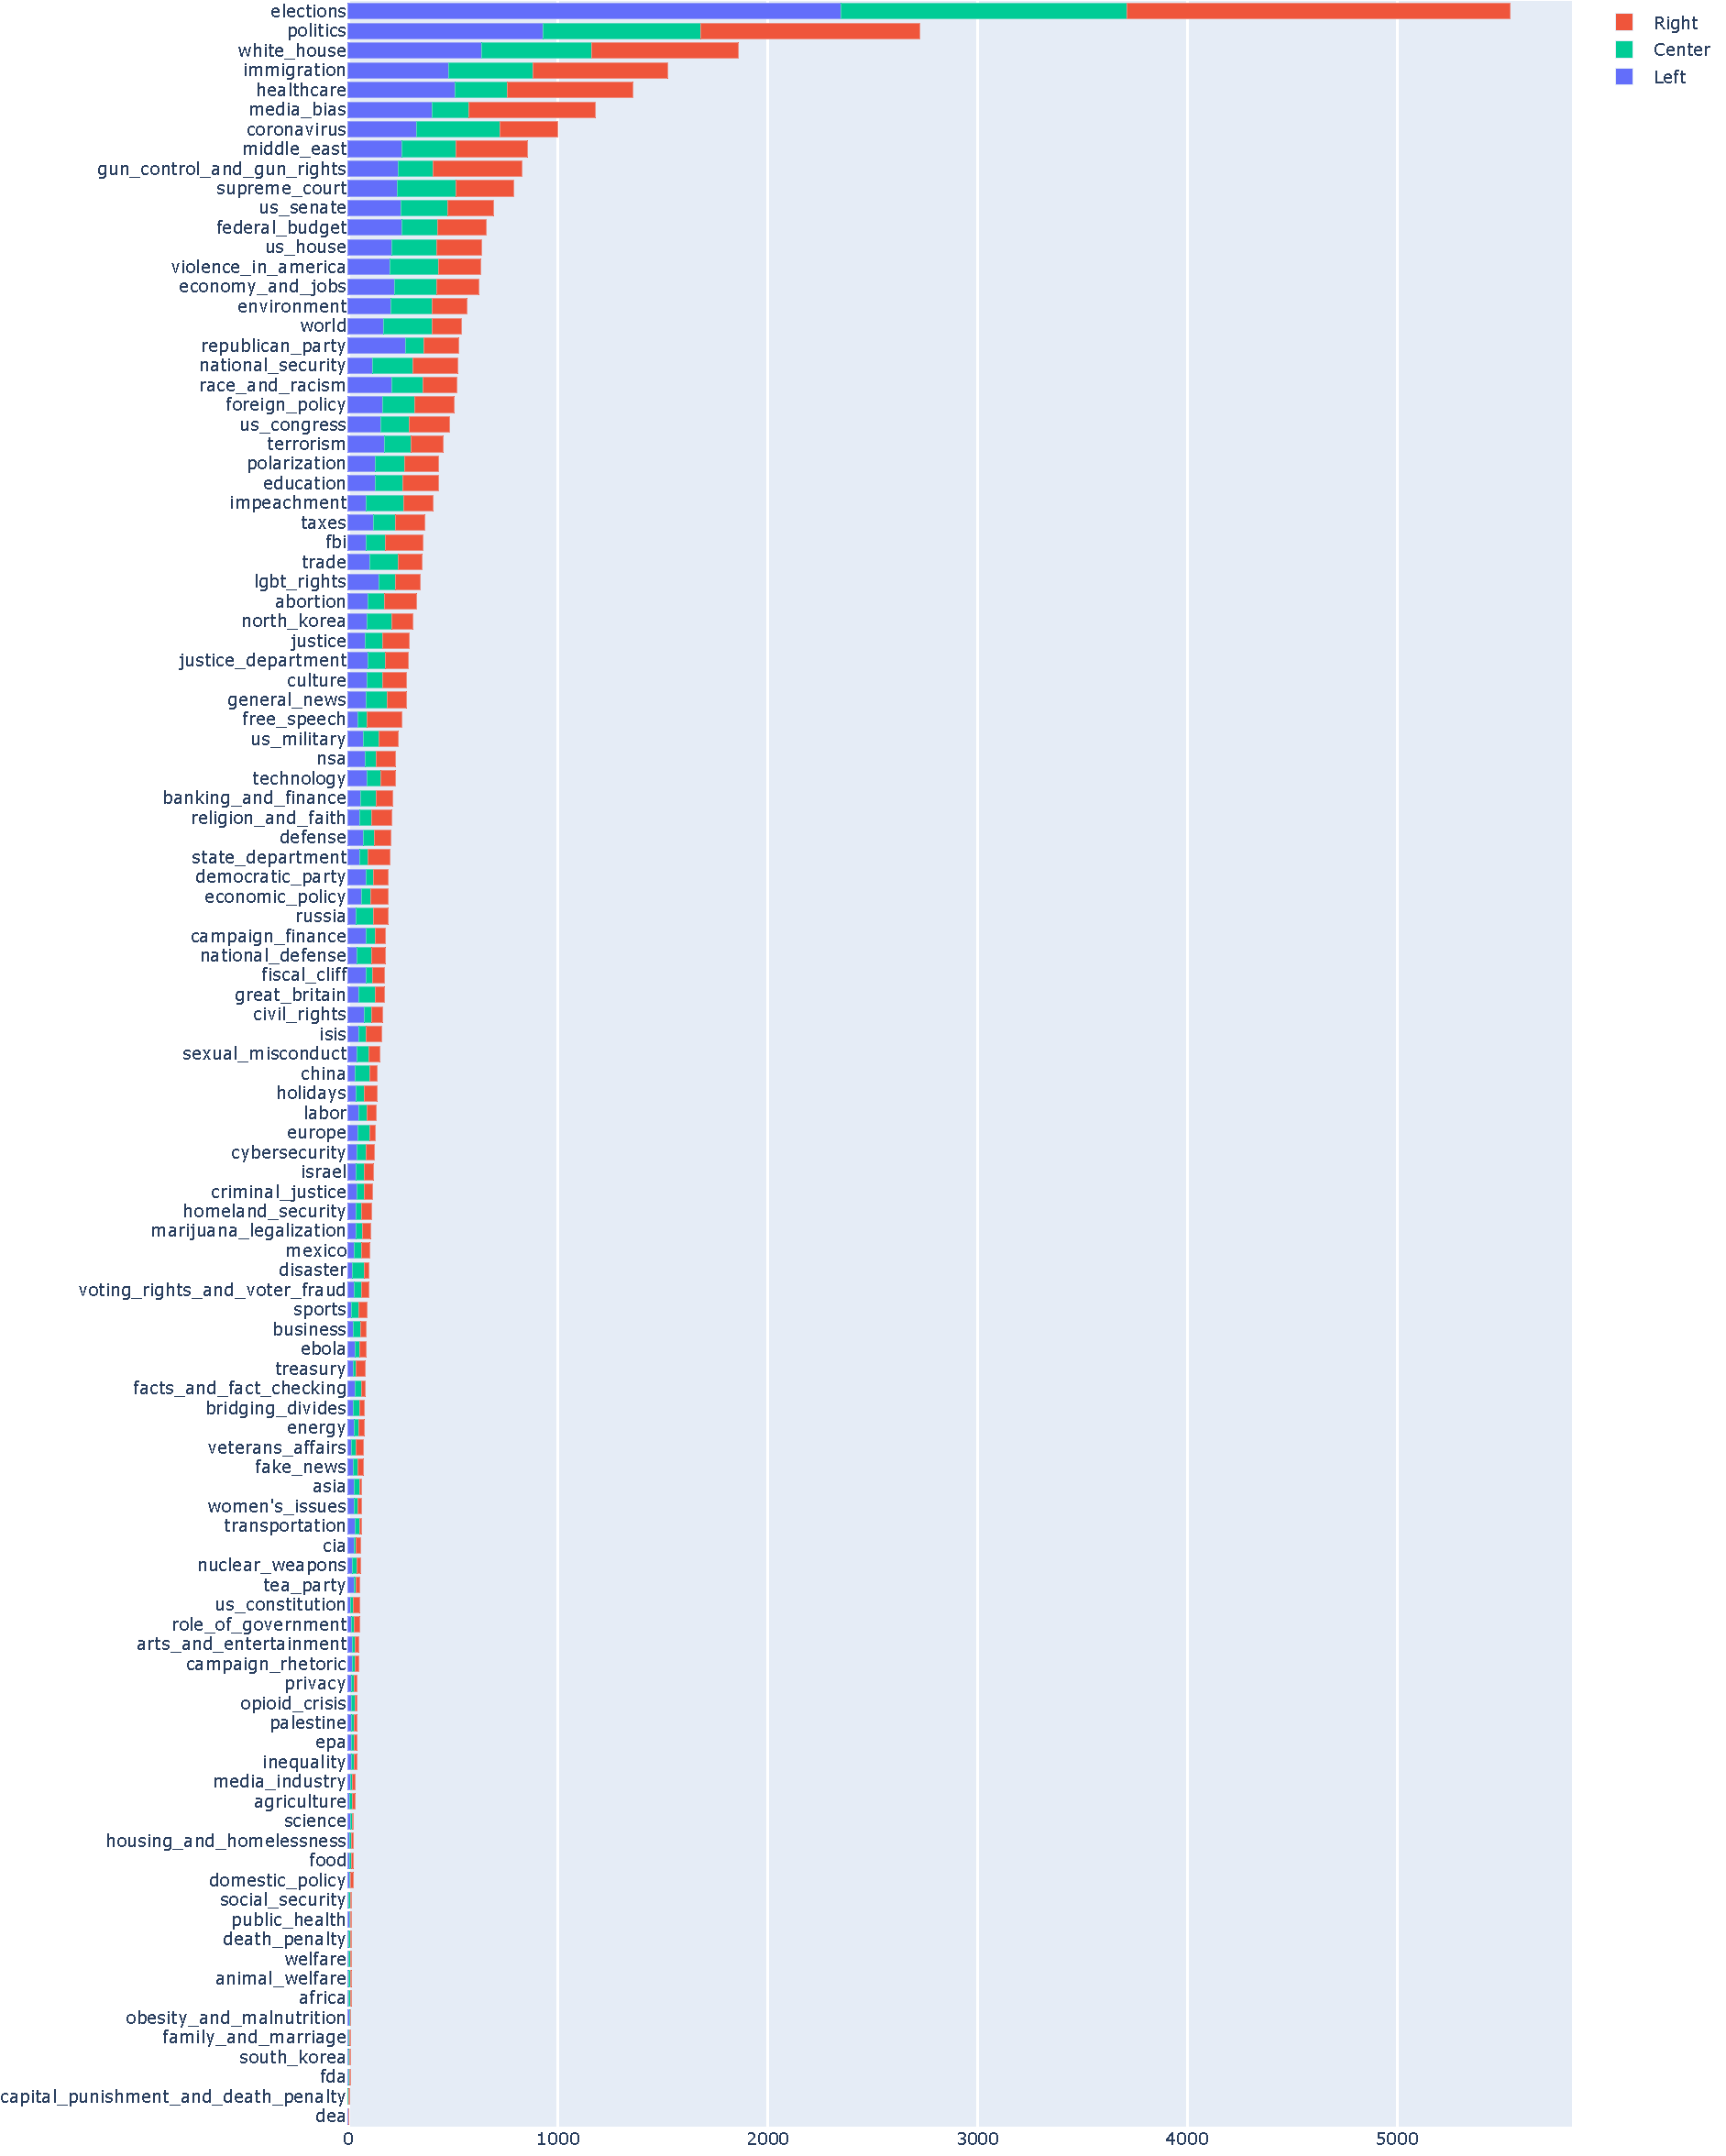
\includegraphics[width=\linewidth]{figures/baly_original_topics_by_leaning.pdf}
    \caption{Original topics of \texttt{Baly} dataset by leaning}
    \label{fig:baly_original_topics_by_leaning}
\end{figure}

Figure~\ref{fig:baly_original_topics_by_leaning} shows that for most of the topics, the quantity does not change significantly across political leaning.
But for some topics, we see something unexpected: there are more articles on a specific leaning. Being the dataset made of triples of articles, we were expecting that everything would have been balanced.
However, the unbalance may be caused by two factors:
\begin{itemize}
    \item some of the triples are made by the AllSides team with unbalanced articles (e.g., two from Left, one from Right)\footnote{\url{https://www.allsides.com/story/greg-craigs-foreign-lobbying-trial-begins}}
    \item during the preparation of the dataset (not available to us) some articles may have been removed because of scraping errors
\end{itemize}

For example, the topics \texttt{gun-control-and-gun-rights}, \texttt{fbi}, \texttt{free-speech}, \texttt{state-department} has more articles on the Right and fewer in the Center. Or the topics \texttt{republican-party}, \texttt{lgbt-rights}, \texttt{civil-rights} that have more articles on the Left.

This confirms that, even though the AllSides team is trying to maintain the balance by displaying all the sides of the news, the imbalance on such topics is so big that in the end they used two articles from the same leaning.

For such topics, the news coverage is very unbalanced if we consider datasets that do not come from AllSides.
One of the main techniques of agenda setting, is deciding what to cover as news and what to ignore. In this way, the perceived importance of issues is manipulated or diverted~\cite{mccombs1972agenda}.

Besides the positive side of this comparison, we cannot infer from this representation the relationships between the different topics.
We know that \texttt{lgbt-rights} and \texttt{civil-rights} are related, but the flat representation of topics does not provide this information.
Furthermore, some topics are too wide and may internally be imbalanced, while some others are very narrow already.

\subsubsection{\statusgreen Coarse Topics}

Instead of using the AllSides topics, here we use the Coarse Topics from TextRazor, that are very broad but at least they are all at the same level (no detailed topics).

\begin{figure}[!htbp]
    \centering
    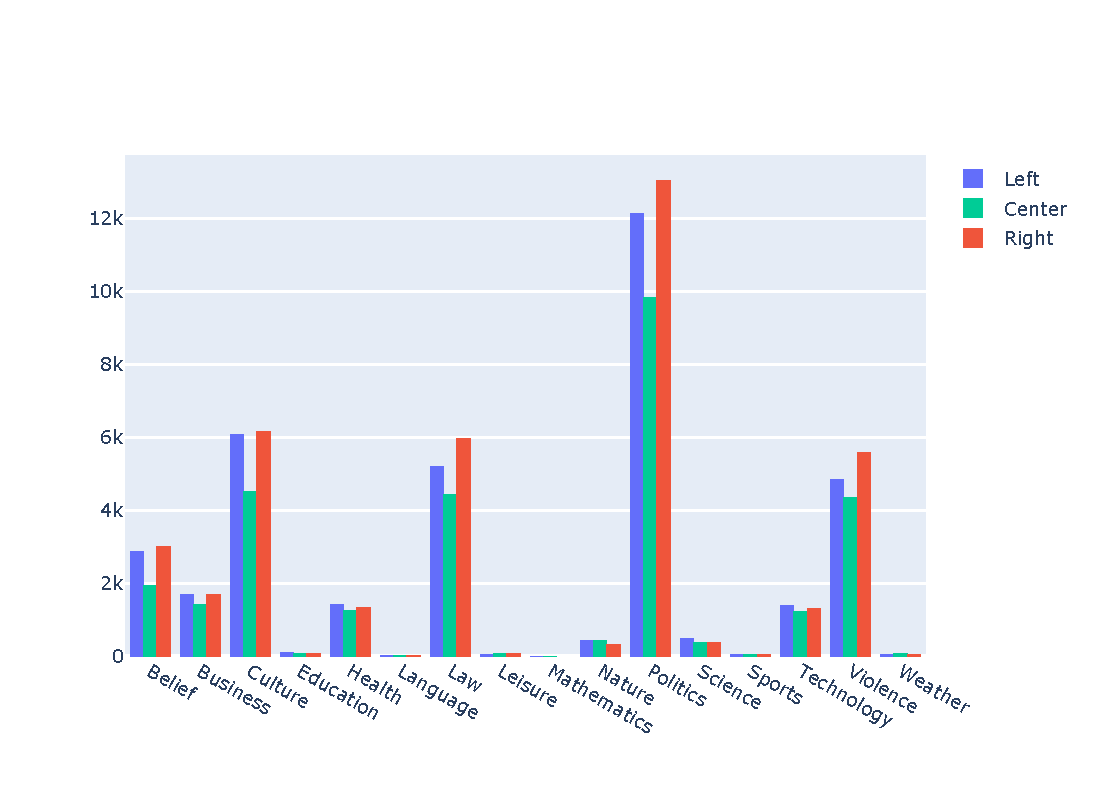
\includegraphics[width=\linewidth]{figures/baly_coarse_weighted_by_leaning.pdf}
    \caption{Coarse Topics weighted of \texttt{Baly} dataset by leaning}
    \label{fig:baly_coarse_weighted_by_leaning}
\end{figure}

Figure~\ref{fig:baly_coarse_weighted_by_leaning} shows the comparison between the different leanings in the dataset with a breakdown by topic.

As in the previous plots representing outputs from TextRazor, we are considering the weights given to the topics of each article (score in the $[0,1]$ interval). The Y-axis is the sum of the topic weights across articles.

With respect to the native topics of AllSides, we have that there are less topics (easier to inspect) but also less differences (does not tell any differences).
While in the previous figure we managed to find some topics with unbalance, here we do not.

The Coarse Topics are not enough granular to see differences across the political spectrum. The only difference that we see, is that there are slightly less articles for the Center in all the topics.

The most prominent topics are Politics, Culture, Law and Violence for all the leanings.

Therefore, we proceed with methods that have more fine-grained topics.

\subsubsection{\statusred Fine-grained topics}

By using the Fine-grained topics of TextRazor, we have the problem of high dimensionality. There are too many topics, and it is very difficult to represent them graphically to find the ones that have the most differences.

\todo{list the top fine-grained topics sorted by support and difference in \% across left-center-right}

\todo{TF-IDF analysis using topic labels to find if some topic terms are more Left or Right}

Still we have the problem of not being able to group topics together and find topic groups that are unbalanced.

\subsubsection{\statusgreen IPTC Media Topics}

We have seen with the previous topic definitions that, if we have topics that are detailed enough, we can start to see some differences of unbalance across leaning.

Using the IPTC Media Topics, we want to be able to see such differences, but at the same time have an idea of how the topics relate.

% Breaking down with respect to topic, is not helpful to find differences between L/C/R if the topic splitting is very unbalanced and very generic.
% When breaking a dataset of news articles we want to have the possibility to break down the topic enough to see differences. 
We want to discover which topics have an unbalanced coverage between Left and Right. In other words, are there topics that are mostly Left or Right?


\begin{figure}[!htbp]
    \centering
    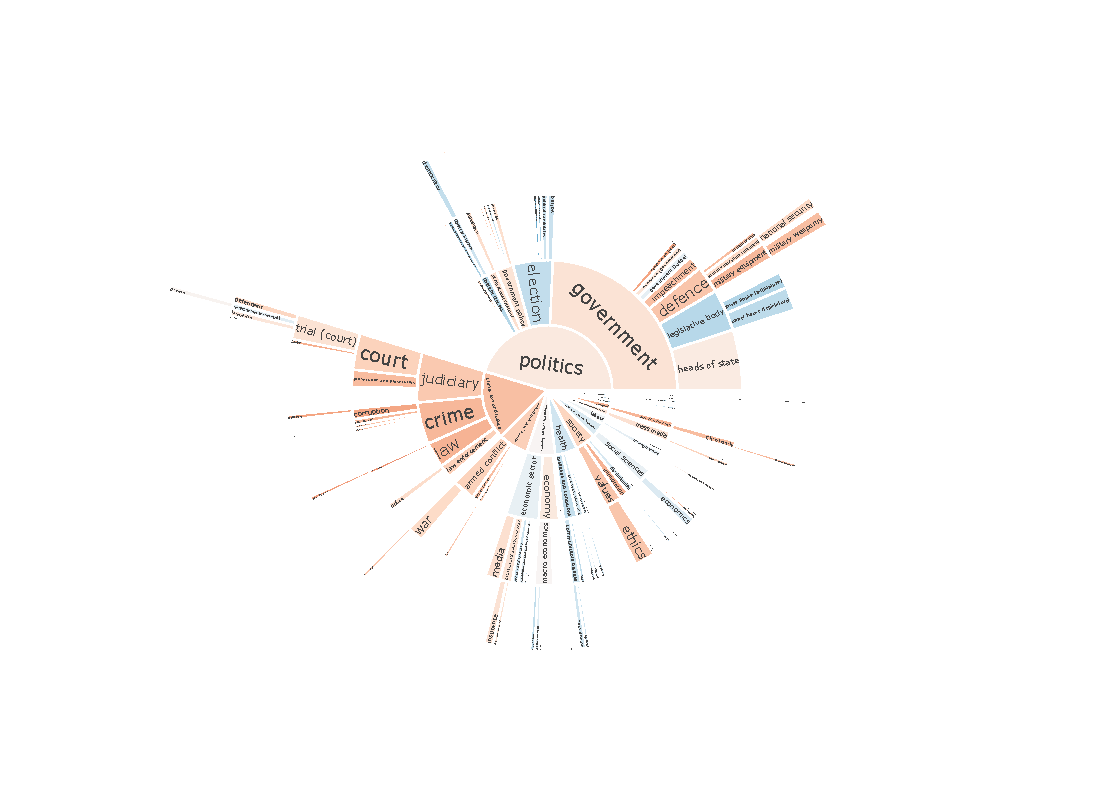
\includegraphics[trim={2.2cm 2cm 2.2cm 2cm},clip,width=\linewidth]{figures/baly_iptc_weighted_by_leaning.pdf}
    \caption{IPTC topics weighted of \texttt{Baly} dataset, average leaning (blue=Left, red=Right)}
    \label{fig:baly_iptc_weighted_by_leaning}
\end{figure}

Figure~\ref{fig:baly_iptc_weighted_by_leaning} shows a Sunburst diagram.\footnote{Interactive chart: \url{https://martinomensio.github.io/phd-project/figures/baly_iptc_weighted_by_leaning.html}}
As in the previous diagram of the same type, the angular distance of each node corresponds to the quantity of that topic in the dataset.
Instead, the colour of the edge is computed with the relative proportion of Left and Right. This means that the colours belong to a scale from blue to red, where blue corresponds to Left while red corresponds to Right.

In this way, we can see with a glance that some topics are covered more by a certain leaning. And we have the information about the hierarchy.

With respect to previous representations, we can see for example that while politics has slightly more articles in the Right (as the dataset all together), the subtopics of elections and legislative body instead appear more in the Left.

\begin{figure}[!htbp]
    \centering
    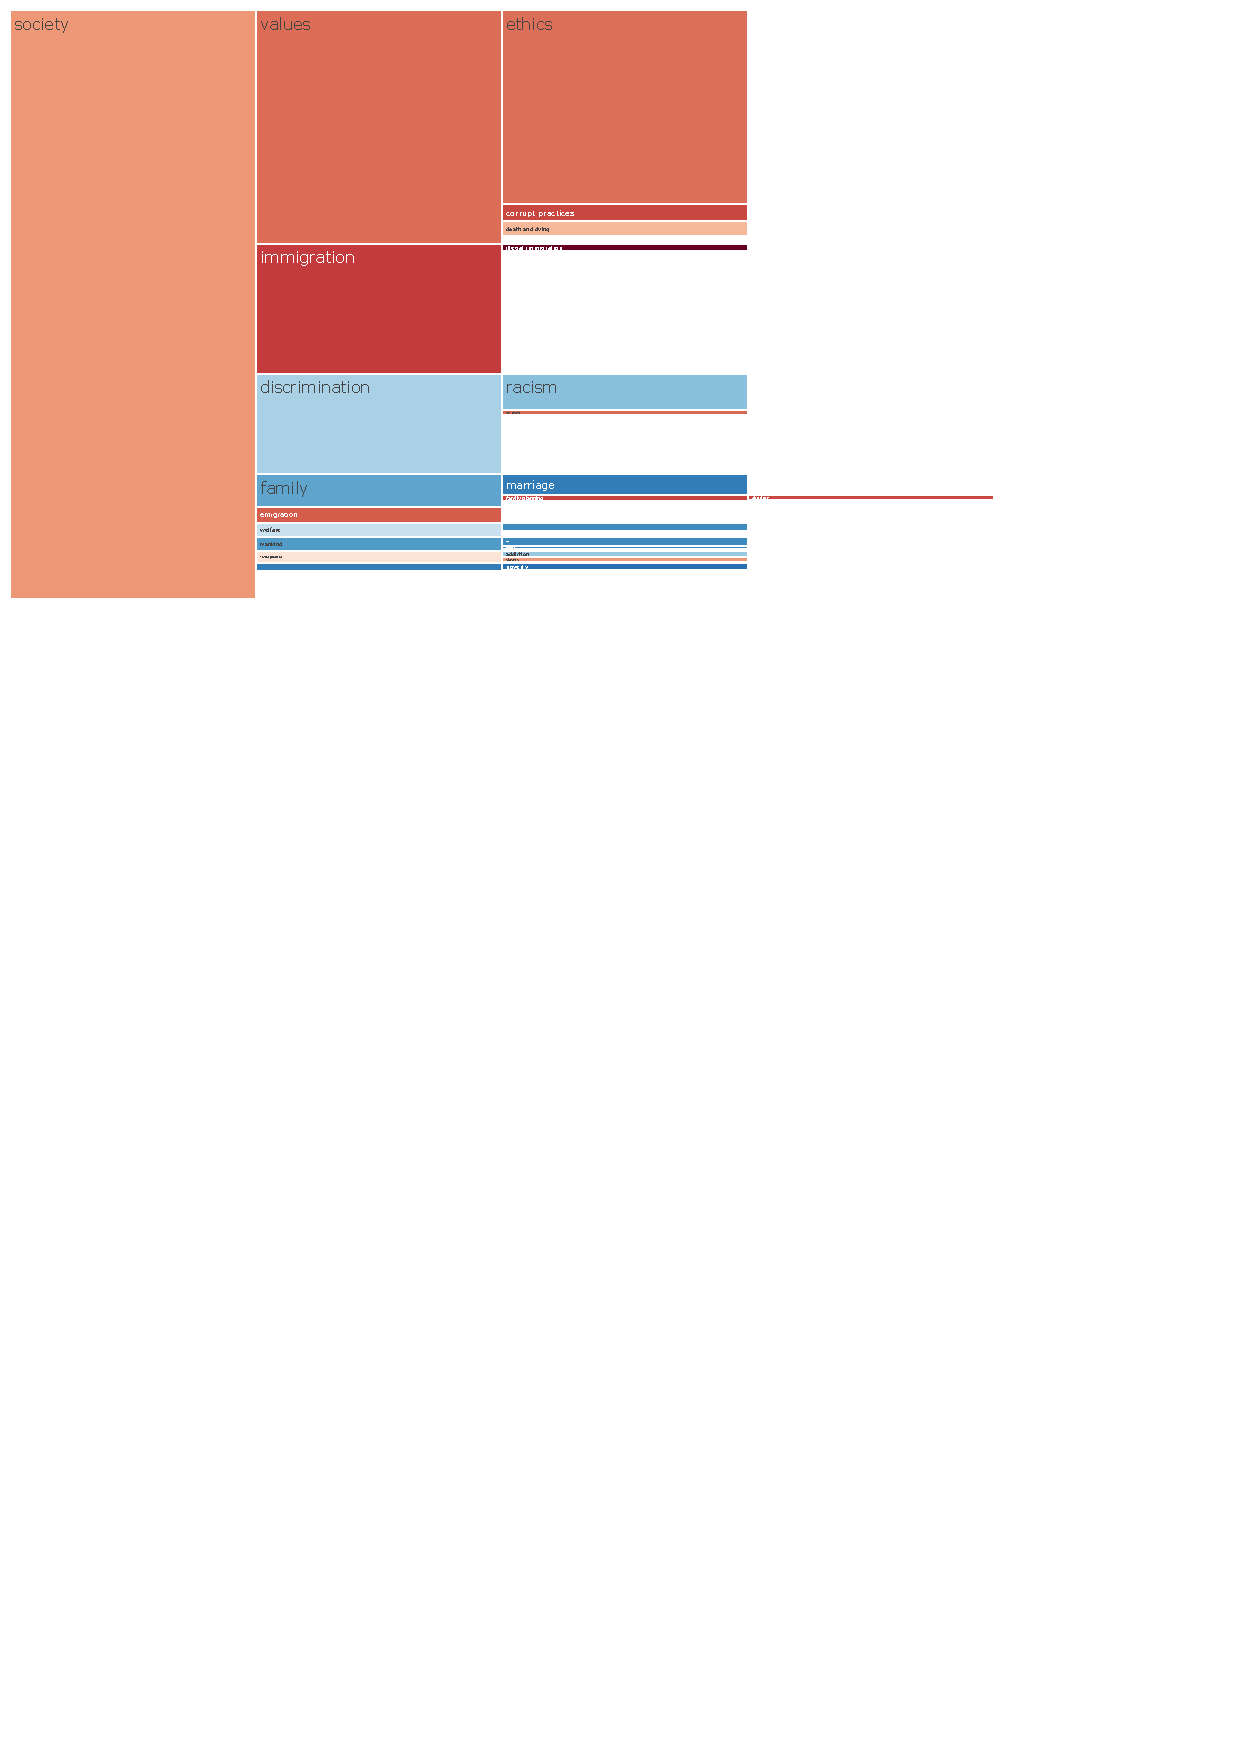
\includegraphics[trim={0 0 0 0},clip,width=0.5\linewidth]{figures/baly_iptc_weighted_by_leaning_zoom_society.pdf}
    \caption{IPTC topics weighted of \texttt{Baly} dataset, average leaning (blue=Left, red=Right), zoom on Society}
    \label{fig:baly_iptc_weighted_by_leaning_zoom_society}
\end{figure}

Or if we interact with \href{https://martinomensio.github.io/phd-project/figures/baly_iptc_weighted_by_leaning.html}{the chart} expanding ``society", we can zoom on the subtopics of society and see as in Figure~\ref{fig:baly_iptc_weighted_by_leaning_zoom_society} that immigration and values are covered more by Right leaning, while discrimination, marriage and LGBTQ are covered more by the Left. 

The main findings from this representation is that the Left is more present in military, crime and war topics. Instead the Left is more centred about health, economy,science, labour, and some very specific subtopics of politics.


\subsection{\statusgreen Selected topic methodology}
\label{ssec:topic_topic_choice}

We have seen in the previous subsections several methodologies for defining and extracting the topics from news articles.

We compared the methodologies by first using the topic information on its own (Subsection~\ref{ssec:topic_topic_granularities_alone}), and then in combination with the political leaning (Subsection~\ref{ssec:topics_topics_leaning}).

We have identified our main needs for our following comparative analysis that will consider propaganda, leaning and topic:

\begin{itemize}
    \item fine-grained topics: to be able to identify differences, that at higher levels are not visible;
    \item finite enumeration: know which labels exist, and not have an infinite number of topics;
    \item defined granularity: knowledge of how coarse each topic is, there are wide topics, together with very narrow ones
    \item hierarchical topics: to explore the relationships (parent/child) between topics
\end{itemize}

% Which one
Given these needs, we identified the IPTC Media Topics as ideal candidates.
% Why
They offer fine-grained topics, that are in finite number (see taxonomy). Furthermore, they define the granularity of the topics, and it is possible to navigate the relationships and observe during a comparative analysis 

In the next sections, we will use only the IPTC Media Topics for carrying our comparative analysis.


\section{\statusgreen Breakdown of propaganda by topics}
\label{sec:topic_propaganda}

With respect to the previous sections, here we bring in the propaganda analysis. As seen in Figure~\ref{fig:methodology_mindmap_chapter6}, the first Research Question (RQ1) is addressing Topics and Propaganda:
\emph{How does the detected propaganda change across the topics?}

To answer this question, we analyse how propaganda is distributed across the topics, to find out which topics contain more propaganda than others (controversial vs non-controversial topics).

We do not take in account political leaning, which is added in the next RQ2.
% and what differences topics contain in terms of propaganda.
% Assumption: propaganda is used for certain topics more than in others

We have the following analysis:

\begin{itemize}
    \item analysis of the total quantity of propaganda across Media Topics: to discover the most controversial/loaded topics (more propaganda) and the non-controversial/unloaded ones;
    \item analysis of the quantity of each propaganda technique across Media Topics: to discover associations of topics and specific techniques;
    % \item analysis of the terms of propaganda across Media Topics: to discover term associations with specific topics.
\end{itemize}

\subsection{Total quantity of propaganda across Media Topics}
\label{sec:topic_propaganda_tot}

% one sunburst with total quantity
From the computed features about each article, here we take the total quantity of propaganda and the Media Topics.
The total quantity of propaganda is a simple percentage that represents the ratio of words that have been annotated as propagandistic by the model presented in~\citet{da2019fine}.
Instead, the Media Topics come in a list with label of the topic and value (interval $[0,1]$).

To compute the average quantity, we iterate over the articles, and for each one of them we see the corresponding propaganda value and the topic values. For each of the topics, we aggregate two different measures: the sum of the topic scores $w_{t_{i},a_{j}}$ (acts as a total counter for that specific topic $t_{i}$ across all the articles $a_{j}$, and is computed as before to create the Sunburst diagrams), and the propaganda scores multiplied for the topic scores $w_{t_{i},a_{j}} \cdot p_{a_{j}}$ ($p_{a_{j}}$ stands for the quantity of propaganda for article $a_{j}$).
For accounting the hierarchy, we propagate these values from the children nodes to their parent nodes, which are summed together ($i\subset k$).
The final average quantity of propaganda for each topic is then computed as:

$$ p_{t_{k}} = \frac{ \sum_{j} \sum_{i\subseteq k} w_{t_{i},a_{j}} \cdot p_{a_{j}} }{ \sum_{j} \sum_{i\subseteq k} w_{t_{i},a_{j}} } $$

\begin{figure}[!htbp]
    \centering
    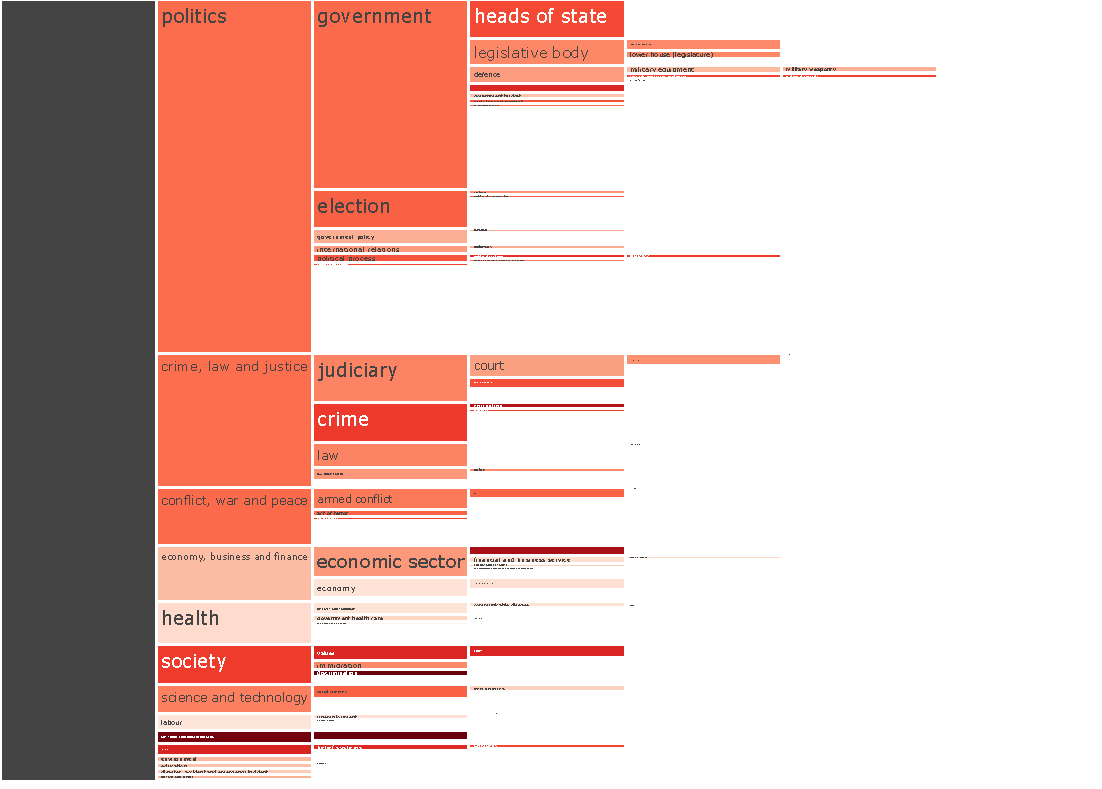
\includegraphics[trim={2.2cm 2cm 2.2cm 2cm},clip,width=\linewidth]{figures/baly_iptc_weighted_prop_total.pdf}
    \caption{Total quantity of propaganda across Media Topics}
    \label{fig:baly_iptc_weighted_prop_total}
\end{figure}

Figure~\ref{fig:baly_iptc_weighted_prop_total} shows the resulting diagram\footnote{Interactive chart: \url{https://martinomensio.github.io/phd-project/figures/baly_iptc_weighted_prop_total.html}} that shows on a redscale (dark red means more propaganda, light red means less) the total quantity of propaganda. To see the values, use the interactive figure.
We can see that the average value is around $5\%$, with the highest ones going slightly above $10\%$.

The topics with most propaganda are: sexism ($9.9\%$) and racism ($9.1\%$), both part of discrimination ($8.1\%$); mass media ($8.0\%$), corruption ($7.2\%$). The lowest values instead are found in economy ($3.5\%$), health ($3.7\%$), government policy ($4.4\%$) and defence ($4.7\%$).

Although we already can distinguish some loaded/controversial topics, we would also like to see the breakdown by specific techniques, therefore in the next subsection we consider each technique individually.

\subsection{Quantity of each propaganda technique across Media Topics}
\label{sec:topic_propaganda_tech}

Similarly to what we have done in Chapter~\ref{chap:linguistic_persuasion}, we want to separate the different techniques. Instead of comparing only the total quantity of propaganda across topics, here we want to see how each of the techniques is distributed across the topics. 

Therefore, when we compute the average quantity of propaganda for the topics, we have to differentiate with respect to the specific technique. In the mathematical formulation, we add from the previous case the technique $m_{l}$ where $l$ is an integer between 1 and 18 that identifies the technique:

$$ p_{t_{k},m_{l}} = \frac{ \sum_{j} \sum_{i\subseteq k} w_{t_{i},a_{j}} \cdot p_{a_{j},m_{l}} }{ \sum_{j} \sum_{i\subseteq k} w_{t_{i},a_{j}} } $$


\begin{figure}[!htbp]
    \centering
    
    

    \centering
	\begin{subfigure}{0.45\textwidth}
		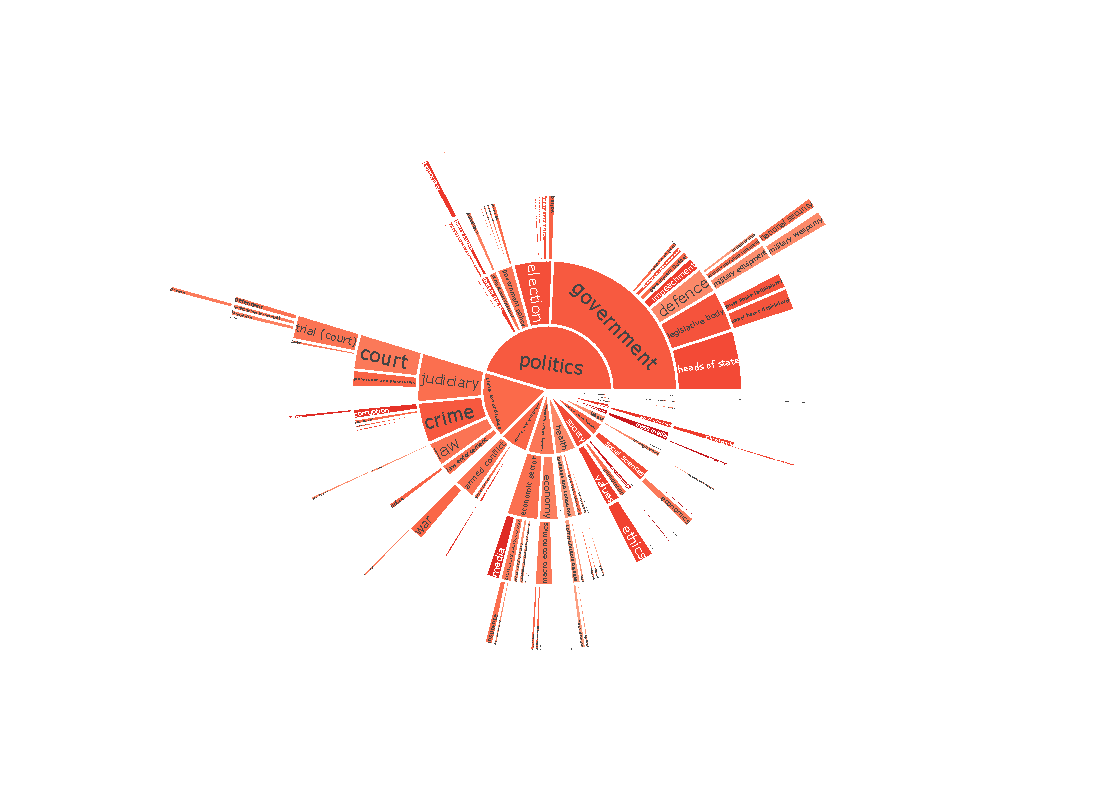
\includegraphics[trim={2.2cm 2cm 2.2cm 2cm},clip,width=\linewidth]{figures/baly_iptc_weighted_prop_tech_Loaded_Language.pdf}
		\caption{Loaded Language}
            \label{fig:baly_iptc_weighted_prop_tech_Loaded_Language}
	\end{subfigure}
	\begin{subfigure}{0.45\textwidth}
		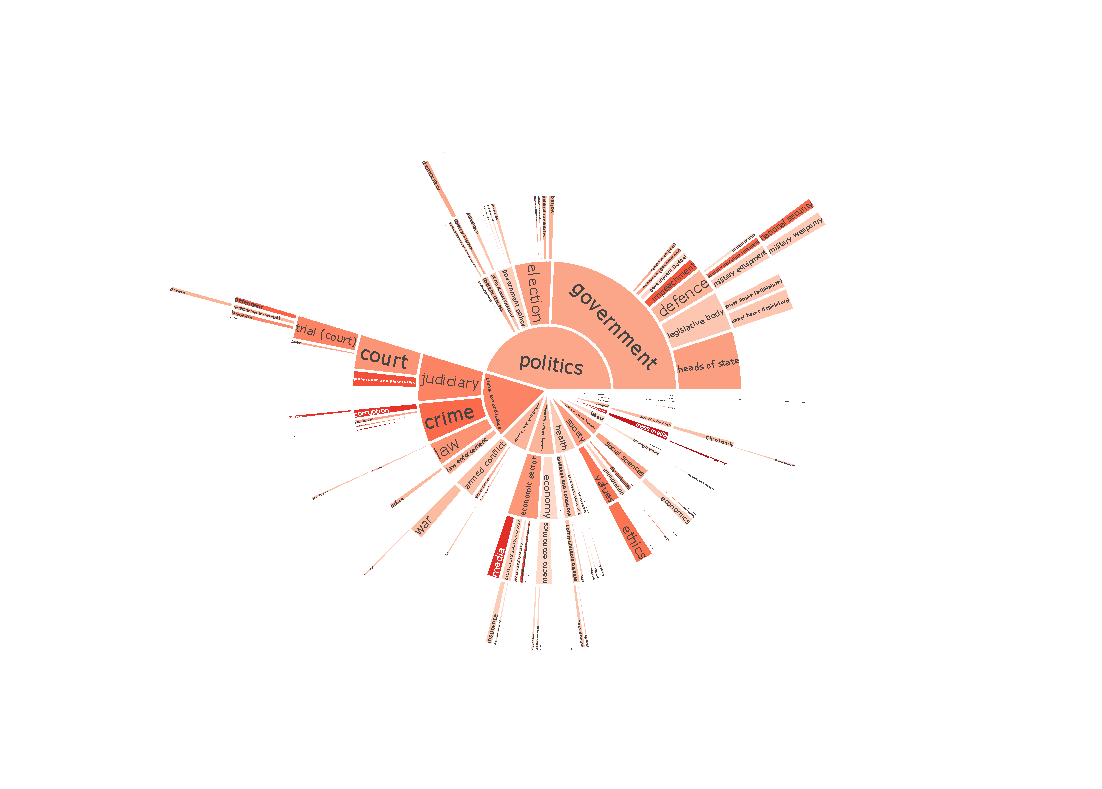
\includegraphics[trim={2.2cm 2cm 2.2cm 2cm},clip,width=\linewidth]{figures/baly_iptc_weighted_prop_tech_Doubt.pdf}
		\caption{Doubt}
            \label{fig:baly_iptc_weighted_prop_tech_Doubt}
	\end{subfigure}
	\begin{subfigure}{0.45\textwidth}
		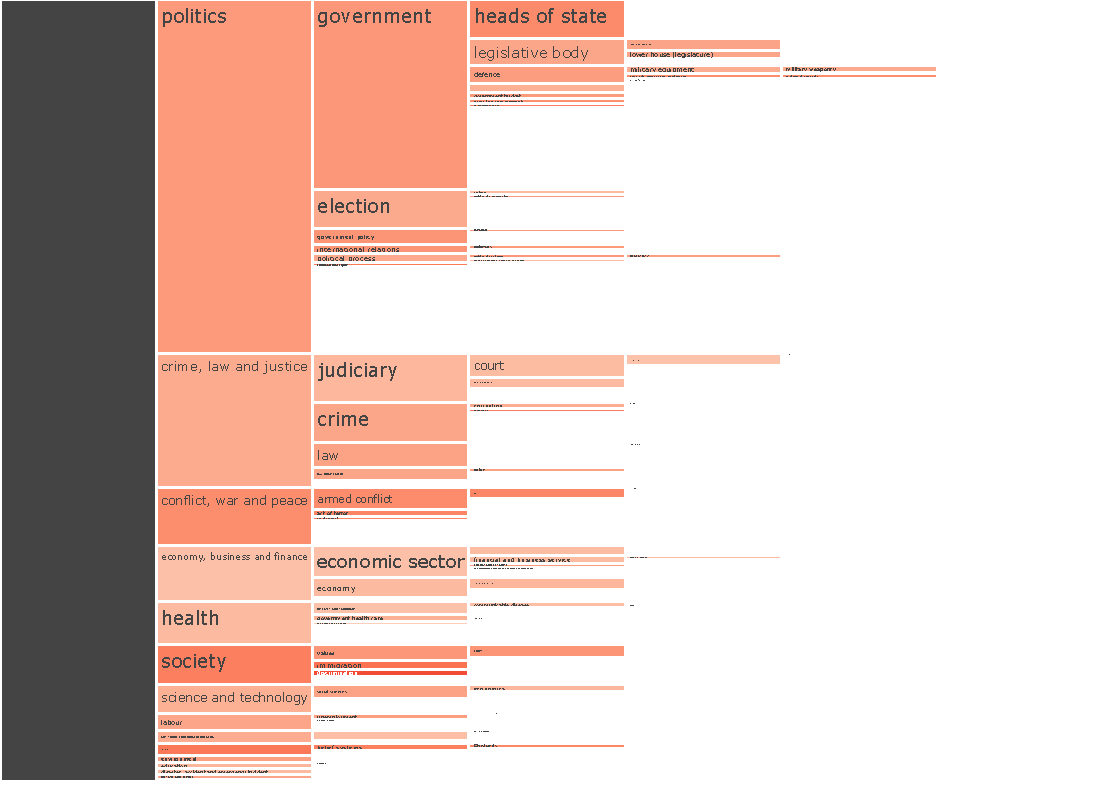
\includegraphics[trim={2.2cm 2cm 2.2cm 2cm},clip,width=\linewidth]{figures/baly_iptc_weighted_prop_tech_Flag-Waving.pdf}
		\caption{Flag-Waving}
            \label{fig:baly_iptc_weighted_prop_tech_Flag-Waving}
	\end{subfigure}
	\begin{subfigure}{0.45\textwidth}
		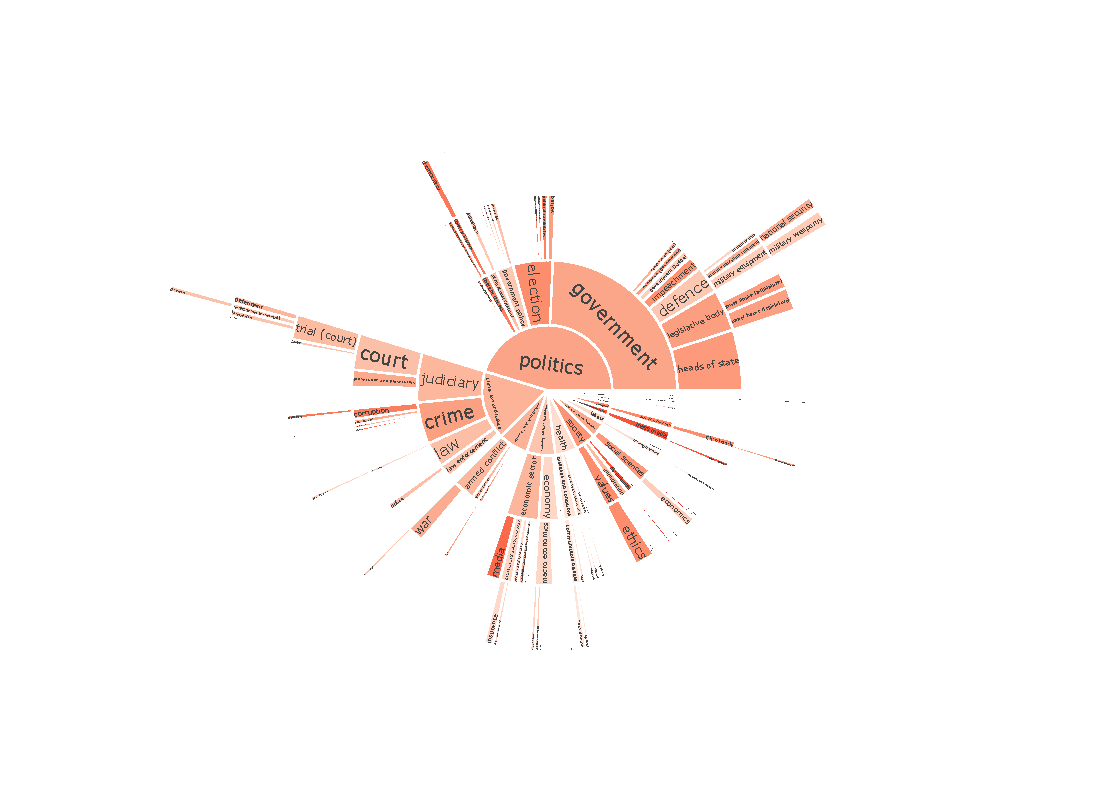
\includegraphics[trim={2.2cm 2cm 2.2cm 2cm},clip,width=\linewidth]{figures/baly_iptc_weighted_prop_tech_Name_Calling-Labeling.pdf}
		\caption{Name Calling / Labeling}
            \label{fig:baly_iptc_weighted_prop_tech_Name_Calling-Labeling}
	\end{subfigure}
	
    \caption{Quantity of propaganda techniques across Media Topics}
    \label{fig:baly_iptc_weighted_prop_tech}
\end{figure}

Figure~\ref{fig:baly_iptc_weighted_prop_tech} shows the four major techniques across Media Topics. We suggest to look at the values on the interactive visualisation\footnote{\url{https://martinomensio.github.io/phd-project/figures/baly_iptc_weighted_prop_tech.html}} where it is possible to select which techniques to visualise, hover on the nodes and see the percentage values, and as well to click on the topics and expand on subtopics.

Here we enumerate, for each technique, the topics where they appear the most:

\begin{enumerate}
    \item Loaded Language: it is the most common technique, as seen in Chapter~\ref{ssec:lp_techniques_propaganda_stats}. Specifically, these topics contain the highest values: Racism ($2.4\%$), Discrimination ($2.2\%$), Mass Media ($2.2\%$) and Corruption ($1.9\%$). These are topics where the opinions are strong and the media uses strong terms to describe the events.
    \item Doubt: as for Loaded Language, Mass Media ($2.2\%$), Corruption ($1.9\%$). Then also Impeachment ($1.65\%$), National Security ($1.5\%$) and Ethics ($1.4\%$). For these topics, we see Doubt as questioning the institutions (especially for Impeachment and National Security).
    \item Flag-waving: Racism ($2.0\%$) and Discrimination ($1.7\%$) as in the previous cases, but uniquely in Religion ($1.3\%$), War ($1.2\%$), Terrorism ($1.3\%$) and Fundamental Rights ($1.3\%$). These are the topics where the nationalism of flag-waving finds the best environment.
    \item Name Calling / Labelling: some topics that emerged also with the previous techniques, such as Mass Media ($1.6\%$), Discrimination ($1.9\%$), Media ($1.4\%$), and Corruption ($1.3\%$). But also Democracy ($1.3\%$) that did not emerge with other techniques. Name Calling uses resonating and evoking terms that fit with topics related to ethical principles.
    \item Appeal to fear / prejudice: the values are quite low, only showing some small strength in Armed Conflict ($0.3\%$), Military Equipment ($0.3\%$) and Communicable Diseases ($0.3\%$). Probably the distributions for Diseases would have been higher if the dataset included more recent events.
    \item Causal Oversimplification: all the values are low, except Discrimination and Racism ($0.4\%$). This makes sense with the nature of the topics, and the news articles treating them may report fallacious reasoning that contains oversimplifications.
    \item Slogans: all values are low, except Civil Unrest ($0.4\%$), Police ($0.2\%$) and Racism ($0.2\%$)
\end{enumerate}

These topic-technique associations verify the theoretical aspects of propaganda and show evidence of patterns that we know from the literature.

% \subsection{Terms of propaganda across Media Topics}
% terms of propaganda by topic?



% \subsection{Coarse Topics}
% \todo{REMOVE SUBSECTION: using coarse topics, heatmaps and no finding: "All three political leanings have very similar profiles, with some exceptions"}

% TextRazor has coarseTopics (up to 5 topics for each article, article-level, e.g. Health/Politics/Law/...) and topics (more fine-grained, around 200 for each article). Each coarseTopic and topic has a weight score which is a value between 0 and 1 representing how prominent is that topic in the article.
% Idea: topic+propaganda techniques
% Which topics are there?
% Which topics co-occur most with propaganda?
% Observe how L/C/R use each propaganda technique in a specific topic



% \subsubsection{Which topics co-occur most with propaganda?}
% This is done at the document level.
% Co-occurrence: heatmap propaganda techniques and topics

% the biggest co-occurrence is between topic violence and technique loaded language.
% BUT it’s only a consequence of Violence and Politics occurring more than other topics in the dataset
% Solution: for each cell divide by the sum of topic quantity. An article can have multiple topics. The values used for the weighting of the matrices are the same for all the rows.

% TODO FIGURE

% (each cell is sum(prop\_quantity*topic\_quantity) / sum(topic\_quantity))
% Each cell represents the average quantity of each propaganda technique for the articles that have been tagged to that topic (considering the topic weight)


% All three political leanings have very similar profiles, with some exceptions

\subsection{Discussion}

Our RQ1 for this section was \emph{How does the detected propaganda change across the topics?}

We have analysed here how propaganda changes across Media Topics, which are our selected methodology from Sec~\ref{sec:topic_topic_granularities}.
First, we analysed which topics contain more propaganda overall (Subsection~\ref{sec:topic_propaganda_tot}), finding a group of topics that are very loaded with propaganda (sexism, racism, discrimination, corruption) and ass well topics with very low values (economy, health, defence).
Then we considered the propaganda techniques individually (Subsection~\ref{sec:topic_propaganda_tech}), and found very specific topic-technique associations.

With this analysis we still do not have a picture of how the political orientation interacts with these loaded areas. Therefore, in the next section / RQ2, we introduce the leaning in the analysis.



\section{\statusred Topic+leaning+propaganda}
\label{sec:topic_propaganda_leaning}

Assumption: propaganda is used for certain topics in a very recognisable way to push for the ideas of the leaning of the source

RQ2: How does the detected propaganda change across topics and leanings? 


Experiment 4.3: 
- topic breakdown: AllSides Topics, IPTC
- shapes of propaganda/sentiment (leaning)


Types of shapes (propaganda)
(look at purple: propaganda)

Blue is sentiment (+ and -) and purple is propaganda. 
y axis in the fraction of terms marked as sentiment/propaganda.

\subsection{Custom Topics (AllSides)}
\todo{REMOVE this subsection. Just check if the main finding is also found with IPTC: Right using Doubt in Science, Center using Appeal to Authority when talking about DEA}

How do they overlap with the propaganda techniques?

Every article is tagged with a topic (AllSides) and with the propaganda techniques (from the tool).
We want to see which topics occur with specific propaganda techniques.
For this reason, we build 3 heatmaps (one for each political leaning) with the propaganda techniques on the x-axis and the topics on the y-axis. The value of the cell represents the average quantity of the propaganda technique for that specific topic.
We want to see differences between the Left/Center/Right heatmaps.

TODO FIGURE: HEATMAP? OR WHAT?

Differences:
The Right is using Doubt when talking about “science” far more than the other two political leanings (1.2\% Left - 13 articles, 0.9\% Center - 8 articles, 5.2\% Right - 4 articles). Does this mean that the Right is more sceptical about science? Let’s look at the data (4 articles from the Right with the topic “science”):
https://spectator.org/science-know-it-alls-on-the-march/
http://www.washingtontimes.com/news/2017/apr/22/march-political-science-earth-day-rally-doubles-la/ 
http://www.nationalreview.com/article/447048/bill-nye-science-guy-march-science-left-politics-religion
https://www.foxnews.com/science/we-could-go-to-venus-with-todays-technology-scientists-say 
The first 3 articles cover the 25 April 2017 march for science, which was labelled by some sources on the Right as “the leftist [...] new religion” (nationalreview article)
3 articles compared here: https://www.allsides.com/story/earth-day-march-science 

The Center is using Appeal to Authority when talking about “dea” far more than the other two leanings (0\% Left - 3 articles, 1.8\% Center - 1 article, 0\% Right - 1 article). Does the Center appeal more to authority because it is more “moderate” than Left and Right?
Other cases can be discovered and the classifier can use them (topic+propaganda technique quantity/terms) to recognise political leaning

\subsubsection{Correlation Left vs Right IPTC}
Exploratory way: observe the correlation between features of the left and features of the right. If correlation is high, it means that the differences are small. Instead if the correlation is low, it means that there exist differences between left and right.


Correlation between L/R of Propaganda quantities (18 values for each article) across topics
The hope is to see that in some subtopics the correlation is low, meaning that the propaganda quantities differ significantly between Left and Right for the subtopic.
On the full dataset, this propaganda feature was not very useful, so let’s see what happens in all the subtopics.

TODO figure sunburst spearmans and pearsons

Scale: blue=correlation high, red=correlation low, grey=not computable (all 0)

This is clearly a negative result. This means that the propaganda quantities are not useful at all. Let’s check what happens with other features:


\subsection{Identifying mediatopics with propaganda differences???}

Objective: using mediatopics taxonomy, find the correct level of narrow that shows differences in how propaganda is used but at the same time not to narrow to still have enough articles.

Differences (quantities of propaganda techniques across leanings), but with enough support. For the sorting it would be nice to have a formula like: 
combined\_score = support(topic) * discrepancy
Or just sort by higher discrepancy, with threshold on support(topic)

Discrepancy computed as correlation?
Distribution of propaganda quantities from L and distribution from R
Option 1: links from AllSides to group the articles in triples
Option 2: average in topic ← selected as doesn’t need info that articles A and B are on the same story. Correlation between quantities of each technique in L vs R

\subsection{Testing on coarseTopic}
Correlation of propaganda techniques quantities between L and R, for each coarseTopic. This is to prove/quantify that coarse topics don’t have much difference in propaganda across political leaning

TODO FIGURE

CoarseTopics that have no high correlation:
Mathematics: pearson=-0.0005, spearman=0.60 (GOOD), support is very small [8. 5. 1.] (BAD)
Language: pearson=0.86, spearman=0.93. Support is [ 83.  48. 109.] articles

Pearson vs Spearman: pearson assumes normal distribution, while Spearman no.
Verifying distribution:

Histogram of quantity of Loaded Language (most prominent technique) of Left (blue), Center (pink) and Right (red) in all the articles. It looks like a normal distribution, truncated at the 0. Y-axis=percentage (TOO: should verify mathematically how close to normal distribution)

\subsection{Fine-Grained Topics}
\todo{REMOVE SUBSECTION: using fine-grained topics but no real result}

Compute for each topic and each leaning, the co-occurrence with each propaganda technique. Then compute the differences (OK with 2 categories, how to do with 3 categories? Variance? But leaning is on a continuum scale), and sort by difference descending → obtain topics with more differences in propaganda quantities
Variance: each observation is the average quantity of propaganda in specific leaning+topic, computed across leaning


:TODO
Then filter and keep only topics with minimum support (to be defined)

How to compare / visualise differences between L/C/R across topics?
Before: heatmaps
Good only for viewing things from the outside, not too fine-grained

What about finding differences by ranking with a function that expresses how much difference is there?
We want topics with high support and have big differences between leaning with respect to a feature (e.g. quantity of a certain technique, term frequencies).

combined\_score = support(topic) * discrepancy

Categorical data comparison?

\subsection{Derived from Entity Types}
\todo{remove}

entity propaganda feature computation
For each entity, compute the total/average propaganda techniques that co-occur in the same sentence by each political leaning. E.g.: “Donald Trump” used a lot of times with “Doubt” from the Left leaning.

Interesting direction:
With Entity linking (provided by TextRazor) it is possible to find common attributes of the entities that make them targets of Left/Right propaganda. E.g., a category of people as repeated target of Propaganda.

\subsection{IPTC Topics quantity}

Top-level IPTC Topics analysis:
Pretty similar to CoarseTopics plot (using native TextRazor 17 categories):
Politics is the most common top-level topic → But this time we will be able to break it down to subtopics (taxonomy)
Crime and conflict also quite relevant
Topics across L/C/R are quite similar → confirmation, the Baly Dataset comes from triples of articles across political spectrum

Then we can cut the hierarchy in any possible way (e.g. top 2 levels)

Right has more propaganda when talking about politics?
Causal Oversimplification higher values in Right
Still not informative: let’s look at the fine-grained mediatopics

Politics breakdown:
politics>fundamental rights + Loaded Language/Slogans: more in Center
politics>fundamental rights>freedom\_of\_religion + Flag-waving: more in Right
politics>government>espionage and intelligence + Doubt: Right

2nd level mediatopics (not only politics)
Plot is not very clear, but shows (topic-technique associations that differ the most):
Human interest>people shows higher flag-waving in the Left articles
Human interest + name-calling in Left articles
Communities + flag-waving in Right

What all this means:
Specific topics, even if they are covered by both Left and Right, they are treated differently in terms of propaganda techniques
Fine-grained topics as an approximation of similarity
Classifier can probably benefit from the interaction between topics and propaganda

Next:
Refine/quantify differences between political leanings → find more topics with different propaganda usage
Term analysis L/C/R with and without considering propaganda





\subsection{IPTC Media Topics correlation}
Idea:
Find mediaTopics that have differences (Pearson/Spearman below a threshold) and have enough articles for each leaning
Compare distributions of these topics

Politics subtopics with either Pearson or Spearman below 0.9

TODO create table with figure from terminal

Nice to see coming up topics such as religion, censorship, veteran affairs, government.
What instead has high correlations? (=is more similar in quantity of propaganda techniques across L/R) → TODO show/represent on the topic tree the areas that are more similar and more different


\subsubsection{Freedom of Religion}
Let’s take an example, e.g. about Freedom of Religion
9 Articles from the Left, 5 from Center, 21 from Right
politics>fundamental rights>freedom of religion: p= 0.7831403727439277 s= 0.7222989890906132 [ 9.  5. 21.]

Looking at the distributions of these 35 articles:

TODO FIGURE

Flag-waving from Right has more flat distribution (higher average too) than Left
TODO: confusing colors, force to 3 standard colors
TODO: maybe it’s not the best way to compare distributions (something like violin plot)



\section{\statusred Leaning classifier}
\label{sec:topic_classifier_propaganda}

RQ3: \emph{What are the effects of combining the propaganda features with the topic features, to recognise the leaning of a news article?}

\subsection{Breakdown by topic}


In this section we aim to analyse the relationship between topics, propaganda and leaning from a different perspective.

First by inspecting F1 across topics, showing which topics are most accurate.
But this does not perform training again, only breaking down by topic the F1 results (which samples are selected.

\todo{IMPORT PLOT}

As figure~\ref{TODO} shows, the F1 metric is very similar across topics.
Although, in some topics it is much higher than the others: X.
In some other topics it is significantly lower.

\todo{INSPECTION OF DATA SAMPLES}



\subsection{Predicting Leaning from topics and propaganda}
\label{sec:topic_classifier_propaganda_2}

7: topics+propaganda for political leaning prediction

\section{\statusred Discussions}
\label{sec:topic_discussion}

Main findings from this chapter:

\begin{enumerate}
    \item we need fine-grained topic to be able to see differences. With coarse topics show similar propaganda across topics leaning. The more we use fine-grained topics, the more differences we are able to see. But at the same time we lose support (less articles specific to the topics, too narrow filters). Need of tradeoff between granularity (see good differences) and support (significance of results). A larger dataset could help.
    \item Topics where propaganda is very different between Left and Right: why is it?
    \item Classifier works better in certain topics
\end{enumerate}


\section{Conclusions}
\label{sec:topic_conclusion}

What is the conclusion of this chapter?